\documentclass[a4paper,12pt]{report}
\usepackage[utf8]{inputenc}
\usepackage[T1]{fontenc}
\usepackage[french]{babel}
\usepackage[babel=true]{csquotes}
\usepackage{mathpazo}
\usepackage{amsmath, amssymb, bm}
\usepackage{geometry}
\geometry{top=2.5cm, bottom=2.5cm, left=2.5cm, right=2.5cm}
\usepackage{setspace}
\onehalfspacing
\usepackage{fancyhdr}
\pagestyle{fancy}
\fancyhf{}
\fancyhead[L]{\nouppercase{\leftmark}}
\fancyhead[R]{\thepage}
\setlength{\headheight}{15pt}
\usepackage{graphicx}
\usepackage{float}
\usepackage{xcolor}
\usepackage{booktabs}
\usepackage{multirow}
\usepackage[font=small,labelfont=bf]{caption}
\definecolor{EMSIblue}{RGB}{0, 119, 182}
\usepackage{titlesec}
\titleformat{\chapter}[display]
  {\bfseries\Large\color{EMSIblue}}
  {\filleft\MakeUppercase{\chaptertitlename} \Huge\thechapter}
  {1ex}
  {\titlerule\vspace{1ex}\filleft}
  [\vspace{1ex}\titlerule]
\usepackage[colorlinks=true, linkcolor=black, urlcolor=blue, citecolor=EMSIblue]{hyperref}

\begin{document}

\begin{titlepage}
    \centering
    \includegraphics[width=0.4\textwidth]{logo_emsi.png} \\[0.5cm]
    {\LARGE \textbf{École d'Ingénieurs - EMSI}} \\[0.5cm]
    \textsc{\Large Rapport Détaillé de Projet de Fin d'Études}\\[0.2cm]
    \rule{\linewidth}{0.5mm} \\[1cm]
    {\huge \bfseries DEEP LEARNING POUR LE DIAGNOSTIC MÉDICAL \\[0.3cm] MULTIMODAL \par}
    \vspace{0.5cm}
    {\Large \textit{Analyse Tabulaire, Radiologique et Textuelle : Étude Théorique et Implémentation}} \\[1cm]
    \rule{\linewidth}{0.5mm} \\[1.5cm]
    \begin{minipage}{0.85\textwidth}
        \centering
        \textit{\textbf{Contexte :} Ce rapport exhaustif documente l'implémentation de réseaux de neurones (MLP, CNN, RNN), d'approches hybrides et de techniques d'explicabilité (XAI) pour l'aide au diagnostic clinique, avec une attention particulière portée aux fondements mathématiques et aux études d'ablation.}
    \end{minipage}
    \vspace{2cm}
    \begin{minipage}{0.45\textwidth}
        \begin{flushleft} \large
            \textbf{Réalisé par :}\\
            Boudour Yassine
        \end{flushleft}
    \end{minipage}
    \hfill
    \begin{minipage}{0.45\textwidth}
        \begin{flushright} \large
            \textbf{Encadré par :}\\
            Mme HIDILA
        \end{flushright}
    \end{minipage}
    \vfill
    {\large Année Universitaire 2025-2026}
\end{titlepage}

\tableofcontents
\newpage
\chapter*{Introduction Générale}
\addcontentsline{toc}{chapter}{Introduction Générale}

Le domaine de la santé connaît une transformation sans précédent portée par la numérisation massive des dossiers médicaux. Aujourd'hui, un patient ne génère plus de simples notes manuscrites, mais un ensemble complexe de données multimodales comprenant des analyses biologiques (données tabulaires), des examens d'imagerie médicale (radiographies, IRM, scanners) et des comptes rendus cliniques détaillés (données textuelles). Cette hétérogénéité d'informations, bien que riche, dépasse souvent la capacité d'analyse humaine rapide et exhaustive. C'est dans ce contexte que l'Intelligence Artificielle, et plus particulièrement le Deep Learning (Apprentissage Profond), s'impose comme un outil incontournable d'aide à la décision clinique.

Ce projet s'articule autour du développement, de l'optimisation et de l'explication de modèles de Deep Learning appliqués à ces trois modalités de données médicales. L'objectif n'est pas de remplacer le médecin, mais de lui fournir un outil d'aide au diagnostic (Computer-Aided Diagnosis, CAD) capable d'analyser d'énormes volumes de données et de mettre en évidence des corrélations subtiles. 

Le présent rapport est structuré de manière à fournir une compréhension approfondie tant théorique que pratique des travaux réalisés. 
\begin{itemize}
    \item \textbf{Le Chapitre 1} pose les fondements mathématiques du Deep Learning nécessaires à la compréhension des architectures utilisées.
    \item \textbf{Le Chapitre 2} détaille l'Analyse Exploratoire des Données (EDA) pour nos trois bases de données : Pima Indians Diabetes, PneumoniaMNIST, et Medical Abstracts.
    \item \textbf{Le Chapitre 3} est consacré au traitement des données tabulaires via les Perceptrons Multicouches (MLP).
    \item \textbf{Le Chapitre 4} explore la vision par ordinateur appliquée à l'imagerie médicale par l'entremise des Réseaux de Neurones Convolutifs (CNN).
    \item \textbf{Le Chapitre 5} traite des données séquentielles et textuelles au moyen des Réseaux de Neurones Récurrents (RNN, LSTM, GRU).
    \item \textbf{Le Chapitre 6} repousse les limites des modèles isolés en proposant des architectures multimodales et hybrides.
    \item \textbf{Le Chapitre 7} aborde la thématique critique de l'explicabilité de l'IA (XAI) en médecine via SHAP, Grad-CAM et LIME.
    \item Enfin, \textbf{Le Chapitre 8} présente une étude d'ablation rigoureuse, validant l'architecture de chaque composant de nos réseaux.
\end{itemize}
\chapter{Fondements Théoriques et Mathématiques du Deep Learning}

L'apprentissage profond s'appuie sur des concepts mathématiques rigoureux issus de l'algèbre linéaire, du calcul différentiel et des probabilités. Ce chapitre dresse un panorama exhaustif des éléments théoriques sur lesquels reposent les modèles développés dans ce projet.

\section{Le Neurone Artificiel}
L'unité de base d'un réseau de neurones est le perceptron. Mathématiquement, un neurone reçoit un vecteur d'entrée $x \in \mathbb{R}^n$, lui applique une transformation affine paramétrée par un vecteur de poids $w \in \mathbb{R}^n$ et un biais $b \in \mathbb{R}$, puis passe le résultat dans une fonction d'activation non linéaire $f$ :
\begin{equation}
y = f\left(\sum_{i=1}^{n} w_i x_i + b\right) = f(w^T x + b)
\end{equation}

\section{Fonctions d'Activation}
L'ajout de non-linéarité est indispensable pour permettre au réseau d'approximer des fonctions complexes (Théorème d'approximation universelle).
\subsection{Sigmoïde et Softmax}
La fonction sigmoïde est particulièrement utile en classification binaire, projetant la sortie dans l'intervalle $]0, 1[$, interprétable comme une probabilité :
\begin{equation}
\sigma(z) = \frac{1}{1 + e^{-z}}
\end{equation}
Pour la classification multiclasse, nous utilisons la fonction Softmax, qui convertit un vecteur de log-vraisemblances en une distribution de probabilités :
\begin{equation}
\text{Softmax}(z_i) = \frac{e^{z_i}}{\sum_{j=1}^{K} e^{z_j}}
\end{equation}
\subsection{ReLU (Rectified Linear Unit)}
Introduite pour pallier le problème de disparition du gradient (vanishing gradient), la fonction ReLU est définie par :
\begin{equation}
\text{ReLU}(z) = \max(0, z)
\end{equation}
Bien qu'elle soit non différentiable en $0$, son calcul est extrêmement rapide et son gradient constant pour $z>0$ accélère la convergence.

\section{Fonctions de Coût (Loss Functions)}
L'entraînement d'un réseau nécessite de quantifier l'erreur de prédiction. 
\subsection{Binary Cross Entropy (BCE)}
Pour les problèmes binaires (ex: détection du diabète), nous minimisons la fonction BCE :
\begin{equation}
\mathcal{L}(y, \hat{y}) = -\frac{1}{N} \sum_{i=1}^{N} \left[ y_i \log(\hat{y}_i) + (1 - y_i) \log(1 - \hat{y}_i) \right]
\end{equation}
\subsection{Categorical Cross Entropy}
Pour les problèmes multiclasses (ex: pneumonie, textes médicaux) :
\begin{equation}
\mathcal{L}(y, \hat{y}) = -\sum_{i=1}^{N} \sum_{k=1}^{K} y_{i,k} \log(\hat{y}_{i,k})
\end{equation}

\section{Rétropropagation et Optimisation}
L'apprentissage s'effectue par la méthode de descente de gradient. L'algorithme de rétropropagation du gradient calcule les dérivées partielles de la fonction de coût par rapport à chaque paramètre du réseau en utilisant la règle de dérivation en chaîne (Chain Rule).
\begin{equation}
W^{(l)} \leftarrow W^{(l)} - \eta \frac{\partial \mathcal{L}}{\partial W^{(l)}}
\end{equation}
Dans ce projet, l'optimiseur \textbf{Adam} (Adaptive Moment Estimation) est massivement utilisé. Adam adapte le taux d'apprentissage de chaque paramètre en utilisant une estimation glissante des premiers et seconds moments des gradients, combinant ainsi les avantages de RMSProp et Momentum.
\chapter{Analyse Exploratoire des Données (EDA)}

La qualité d'un modèle d'Intelligence Artificielle est intrinsèquement liée à la qualité des données sur lesquelles il a été entraîné. L'adage "Garbage In, Garbage Out" prend tout son sens en milieu médical, où une donnée biaisée peut entraîner un diagnostic erroné aux conséquences dramatiques. Ce chapitre est dédié à l'Analyse Exploratoire des Données (EDA) pour comprendre la structure, les distributions, les corrélations et les anomalies de nos trois jeux de données.

\section{Jeu de Données Tabulaire : Pima Indians Diabetes}
Le dataset Pima Indians Diabetes recueille des informations physiologiques et cliniques sur 768 femmes d'origine Pima (Amérindiennes). L'objectif est de prédire l'apparition du diabète sucré de type 2 d'ici 5 ans.

\subsection{Description des Variables}
Le dataset comporte 8 variables prédictives (features) continues ou discrètes, et une variable cible binaire (Outcome).
\begin{itemize}
    \item \textbf{Pregnancies} : Nombre de grossesses.
    \item \textbf{Glucose} : Concentration plasmatique de glucose à 2h (test de tolérance au glucose).
    \item \textbf{BloodPressure} : Pression artérielle diastolique (mm Hg).
    \item \textbf{SkinThickness} : Épaisseur du pli cutané tricipital (mm).
    \item \textbf{Insulin} : Insuline sérique sur 2 heures (mu U/ml).
    \item \textbf{BMI} : Indice de Masse Corporelle (poids en kg / (taille en m)$^2$).
    \item \textbf{DiabetesPedigreeFunction} : Fonction qui évalue la probabilité de diabète selon l'historique familial.
    \item \textbf{Age} : Âge en années.
\end{itemize}

\subsection{Problèmes Qualitatifs et Prétraitement}
L'analyse statistique initiale a révélé la présence de valeurs nulles (zéros) biologiquement inconcevables pour les variables \textit{Glucose, BloodPressure, SkinThickness, Insulin} et \textit{BMI}. Il s'agit en réalité de valeurs manquantes encodées par erreur à zéro.
Pour y remédier, nous avons appliqué une stratégie d'imputation en remplaçant ces zéros par la médiane de la variable cible par rapport à la classe (diabétique ou non). La médiane est préférée à la moyenne pour sa robustesse face aux valeurs aberrantes (outliers).

\subsection{Analyse Multivariée et Corrélations}
La matrice de corrélation linéaire de Pearson a été calculée pour identifier les dépendances linéaires. Le glucose présente la plus forte corrélation positive avec l'issue (r = 0.47), suivi de l'IMC (r = 0.29) et de l'âge (r = 0.24). L'insuline et l'épaisseur cutanée sont également corrélées (multicolinéarité).

\begin{figure}[H]
    \centering
    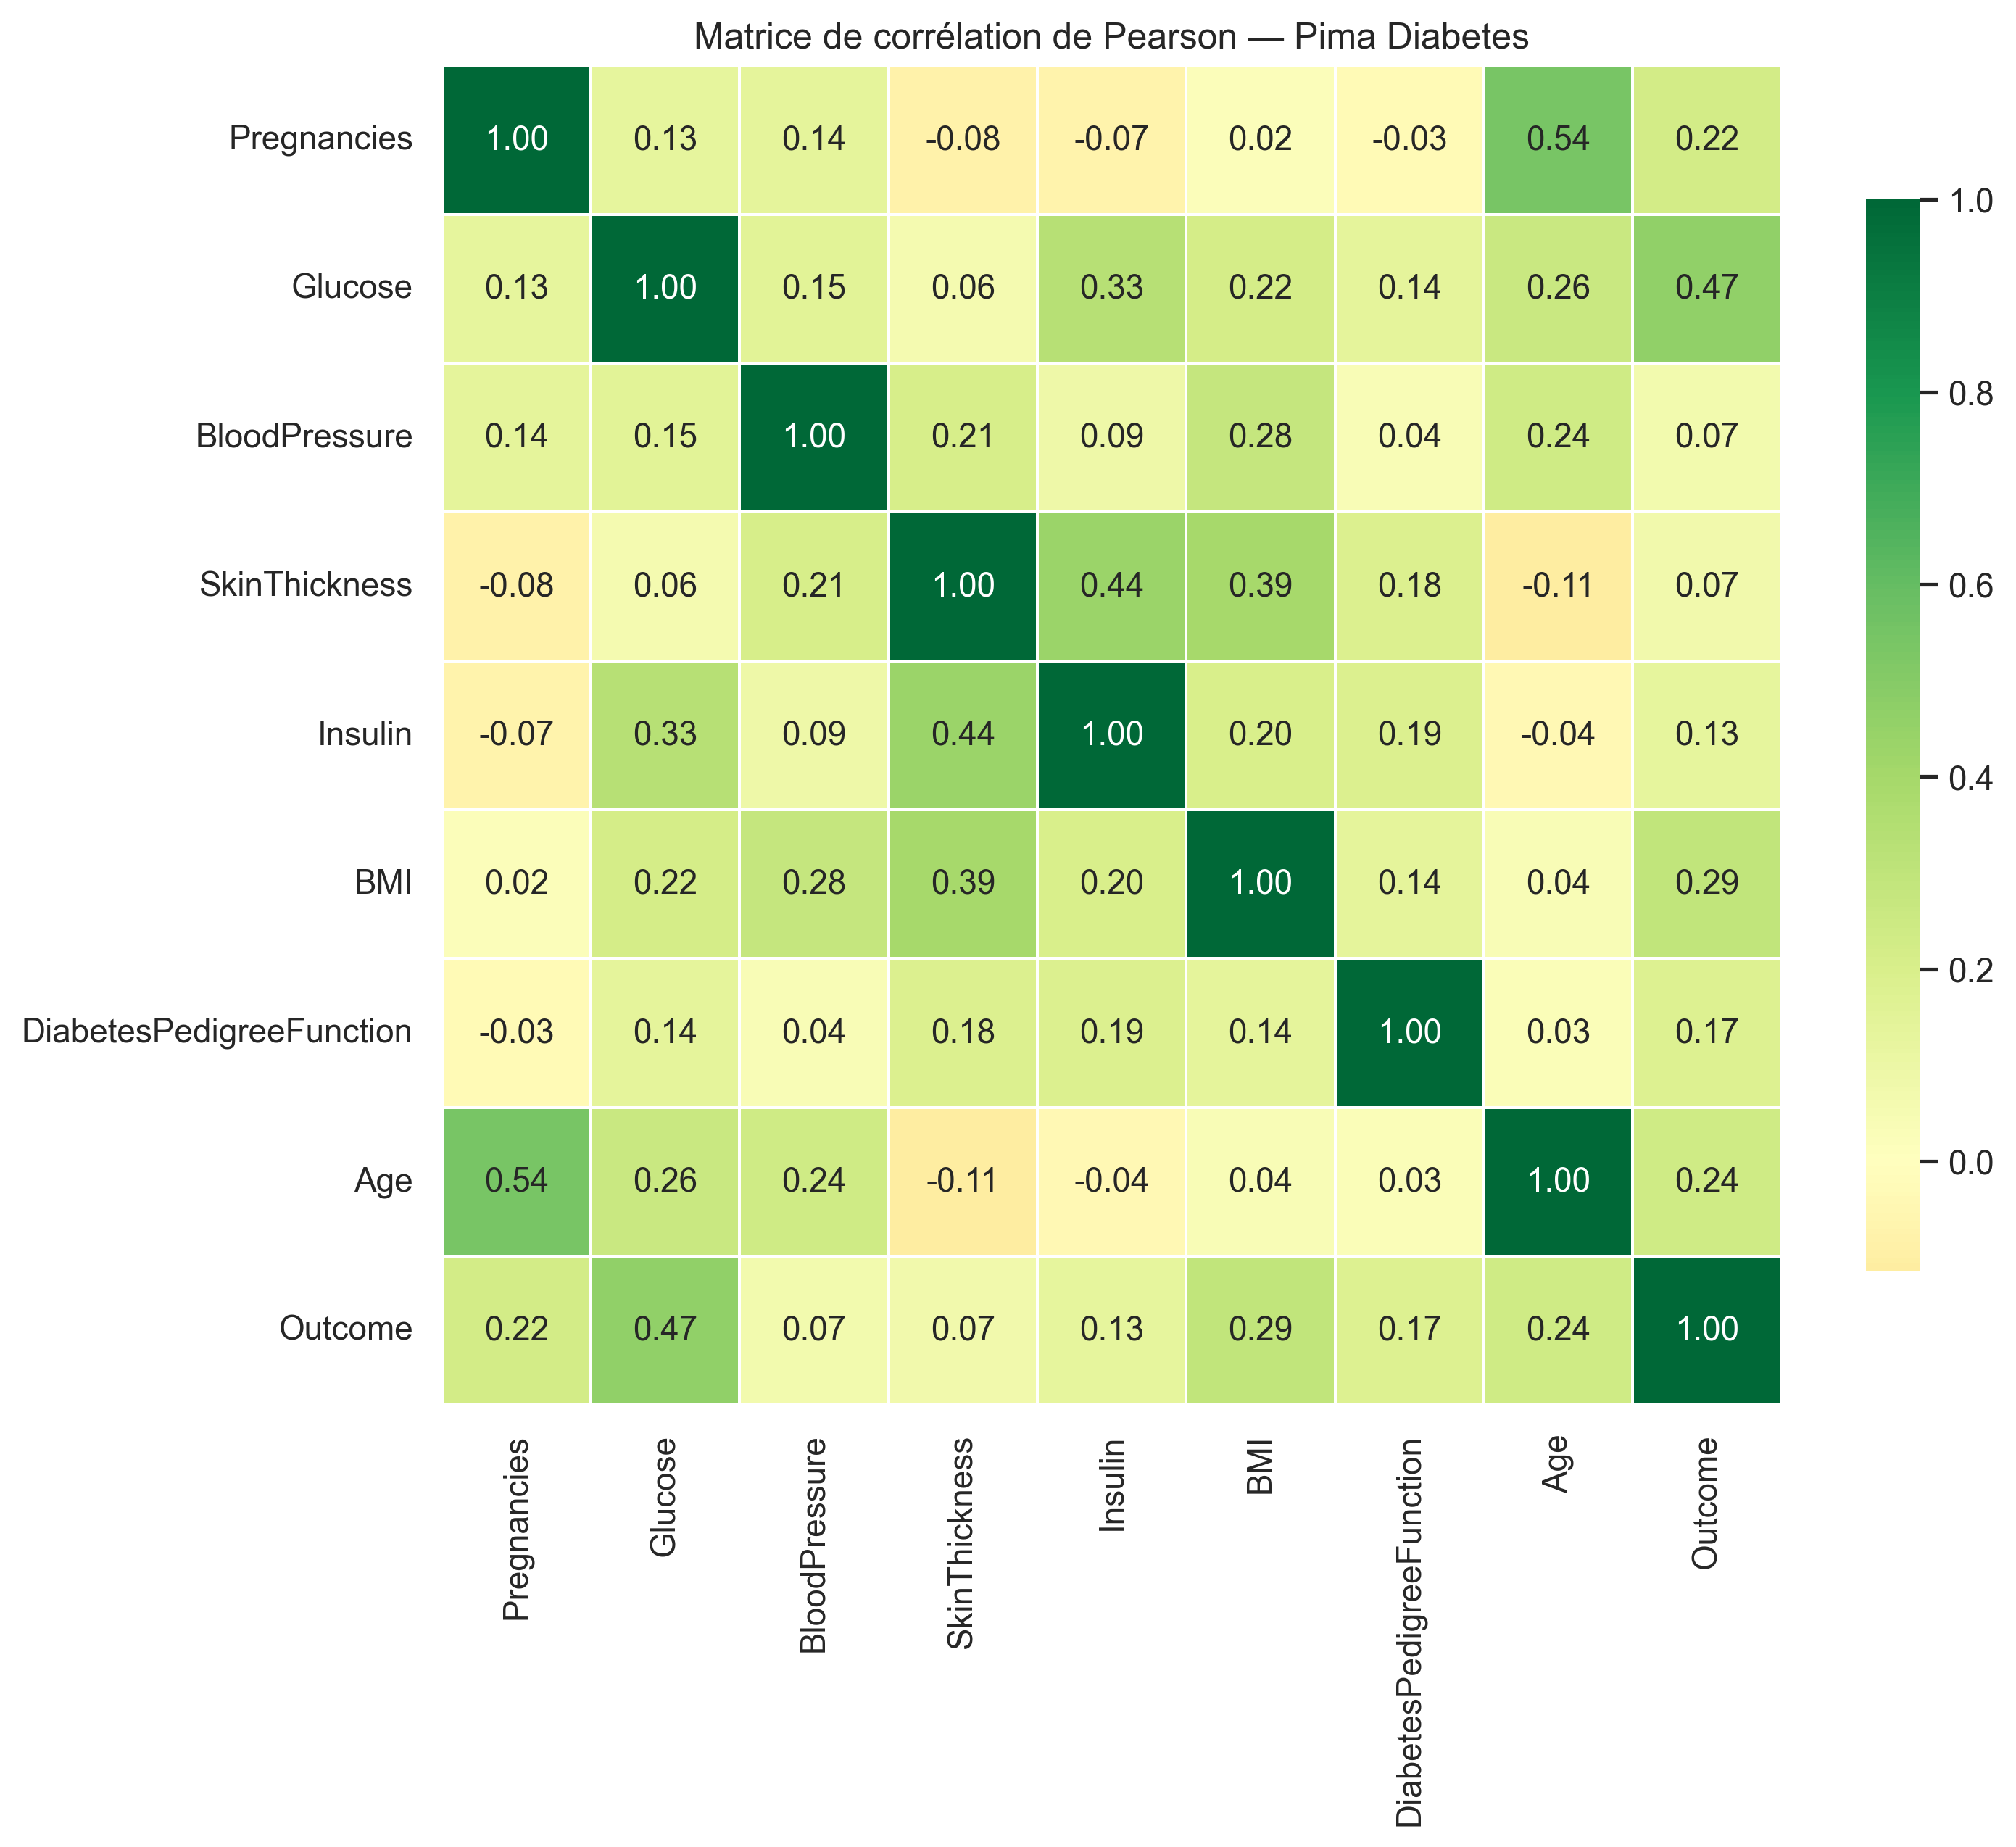
\includegraphics[width=0.85\textwidth]{pima_corr_full.png}
    \caption{Matrice de corrélation complète du dataset Pima Indians Diabetes}
\end{figure}

Les distributions conditionnelles (Boxplots et Violinplots) ont révélé un chevauchement significatif entre les classes "Sain" et "Diabétique". Cette non-séparabilité linéaire parfaite justifie l'utilisation d'architectures non-linéaires profondes (MLP) plutôt que de simples régressions logistiques.

\begin{figure}[H]
    \centering
    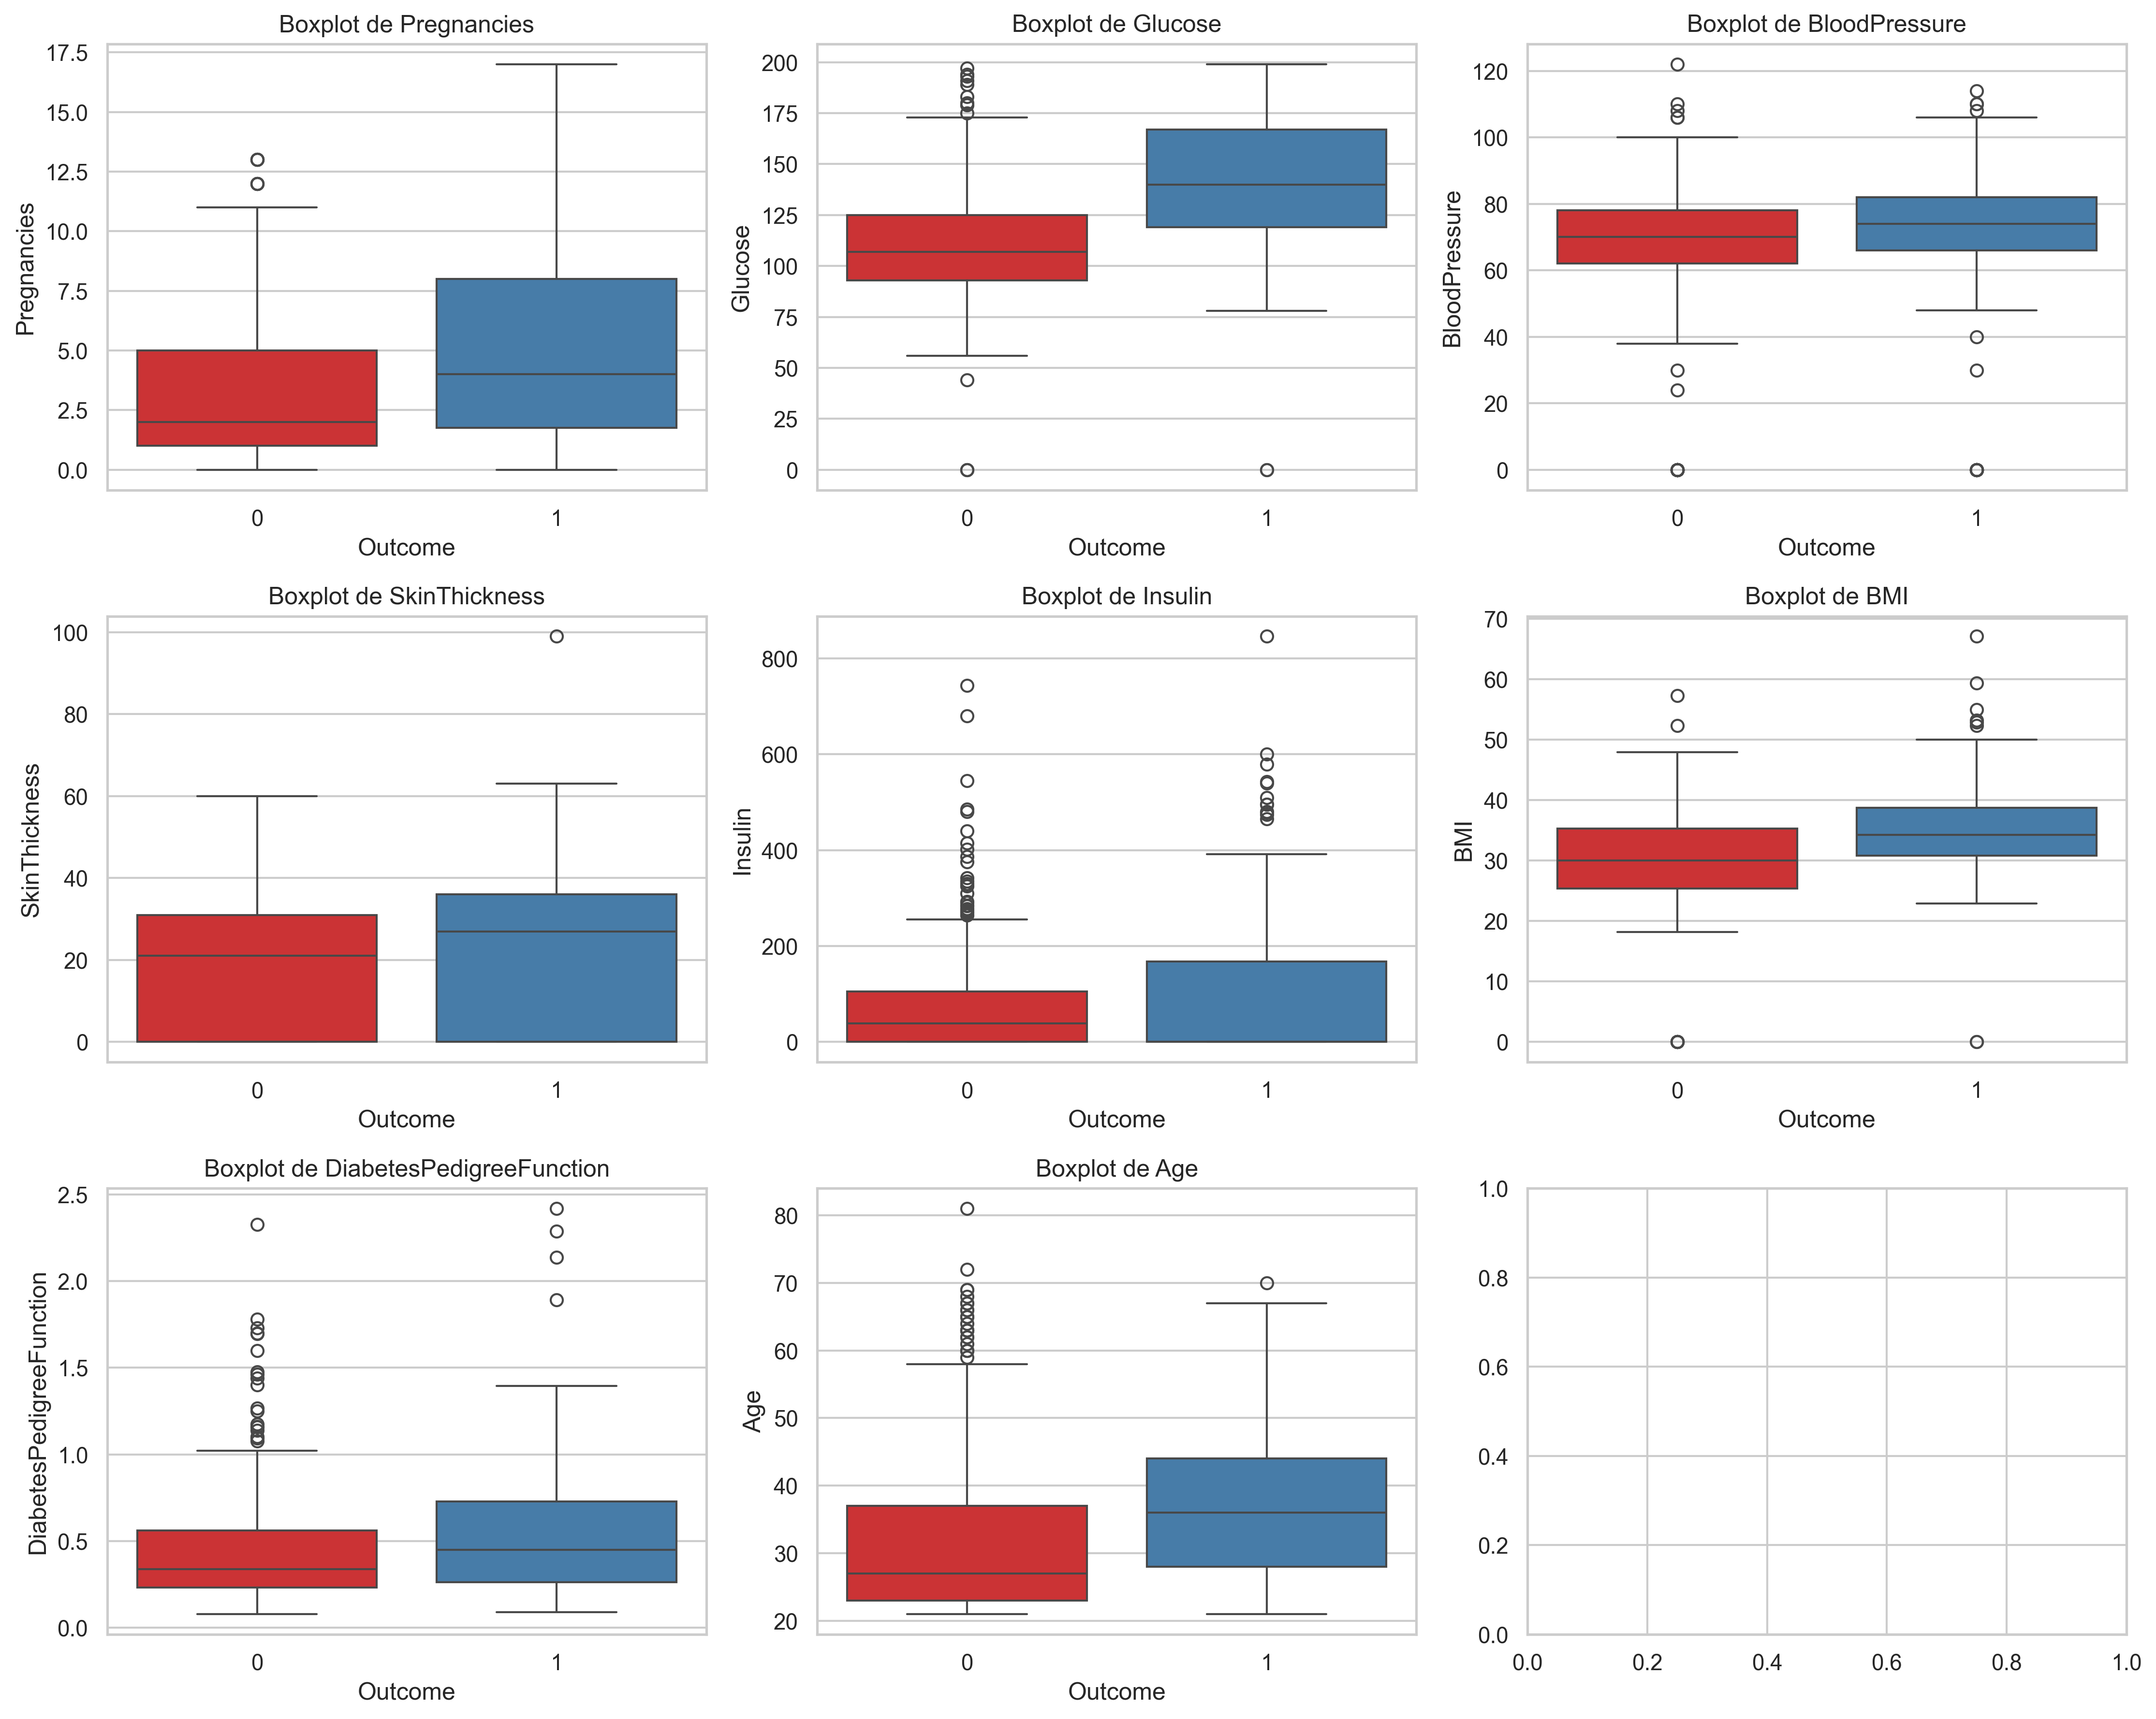
\includegraphics[width=0.85\textwidth]{pima_boxplots.png}
    \caption{Distribution par Boxplot des variables cliniques selon l'issue}
\end{figure}

\begin{figure}[H]
    \centering
    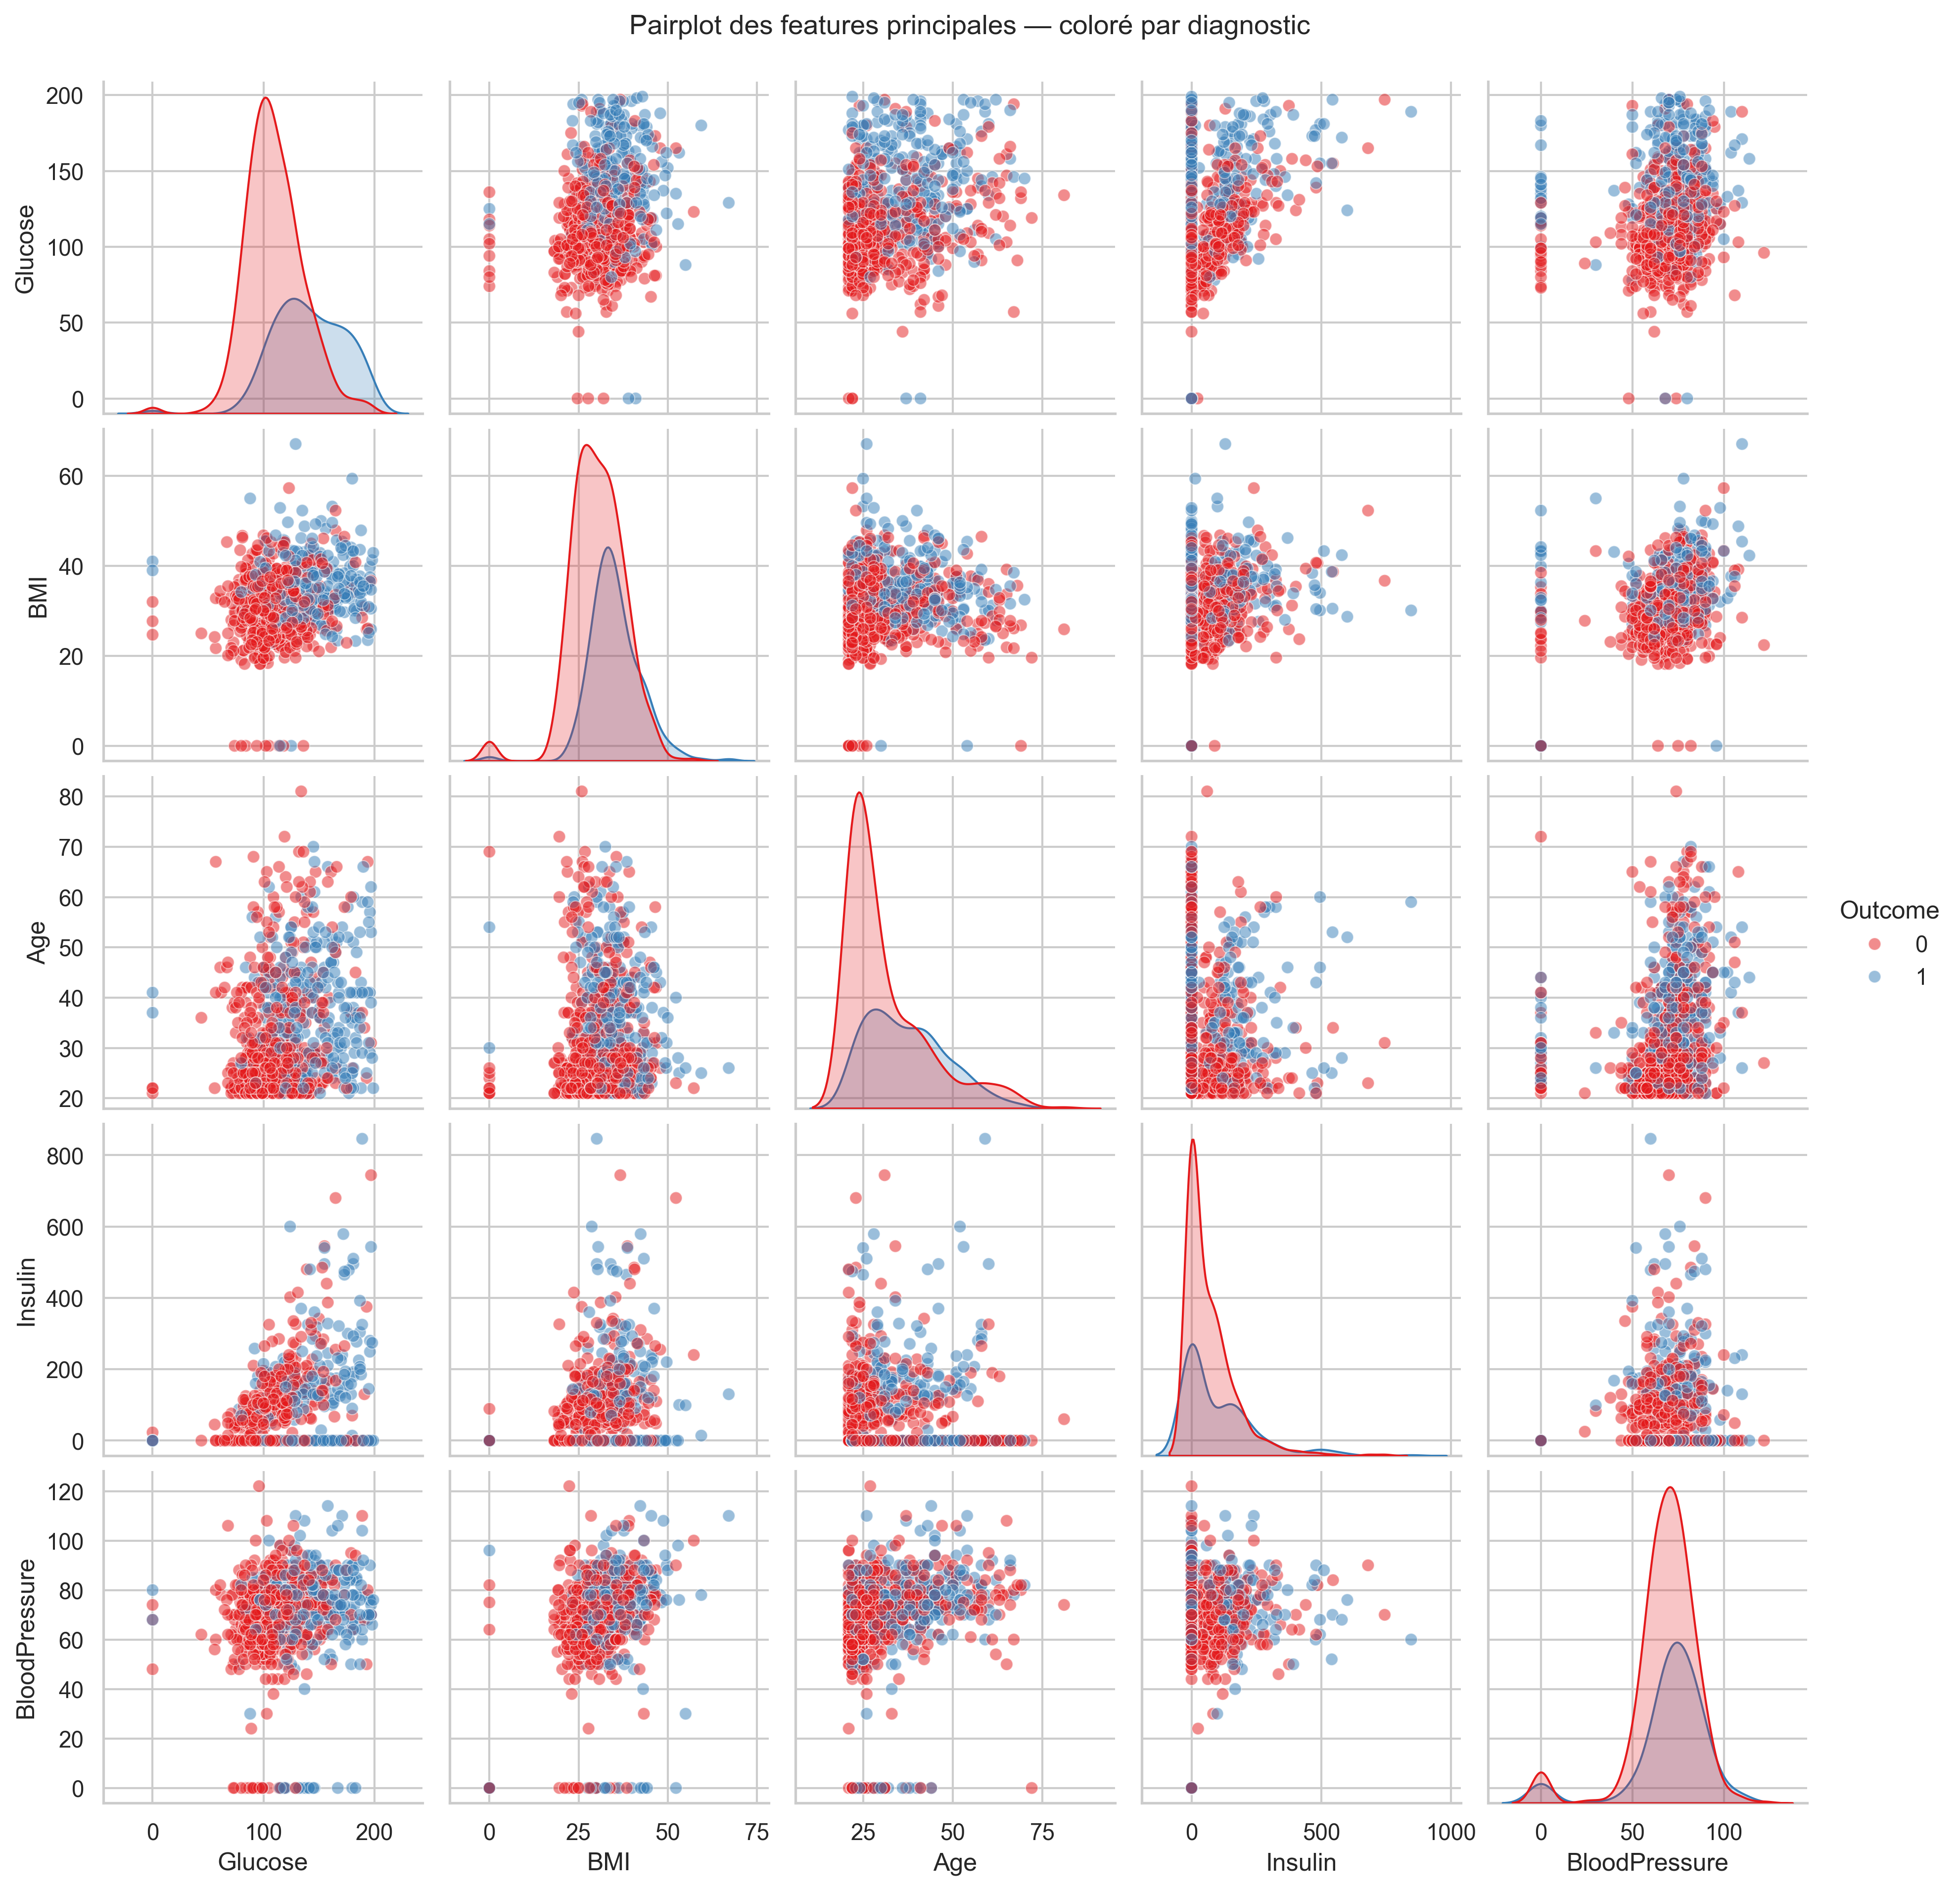
\includegraphics[width=0.85\textwidth]{pima_pairplot.png}
    \caption{Pairplot : Nuages de points croisés pour les variables majeures}
\end{figure}

\section{Jeu de Données Radiologique : PneumoniaMNIST}
Dans le cadre de l'initiative MedMNIST, ce dataset standardisé propose des radiographies thoraciques pédiatriques de format 28x28 pixels en niveaux de gris, dédiées à la classification binaire : Poumons sains (Normal) vs Poumons infectés (Pneumonia).

\subsection{Répartition et Équilibrage}
Le jeu de données comprend 5 856 images réparties en sous-ensembles de Train, Validation et Test. Une analyse de la distribution révèle un fort déséquilibre de classes (environ 74\% de pneumonies). Ce biais naturel (la majorité des patients passant une radio présentent des symptômes cliniques) impose l'utilisation d'une fonction de coût pondérée ou de métriques d'évaluation robustes comme le F1-Score et l'AUC-ROC, l'Accuracy globale pouvant être trompeuse.

\subsection{Analyse Visuelle et Pixel-wise}
Les radiographies révèlent visuellement des différences physiologiques :
\begin{itemize}
    \item \textbf{Normal} : Clarté des champs pulmonaires, contour net de la silhouette cardiaque, angles costodiaphragmatiques dégagés.
    \item \textbf{Pneumonie} : Opacifications alvéolaires, consolidations diffuses ou lobaires, oblitération des contours cardiaques.
\end{itemize}

\begin{figure}[H]
    \centering
    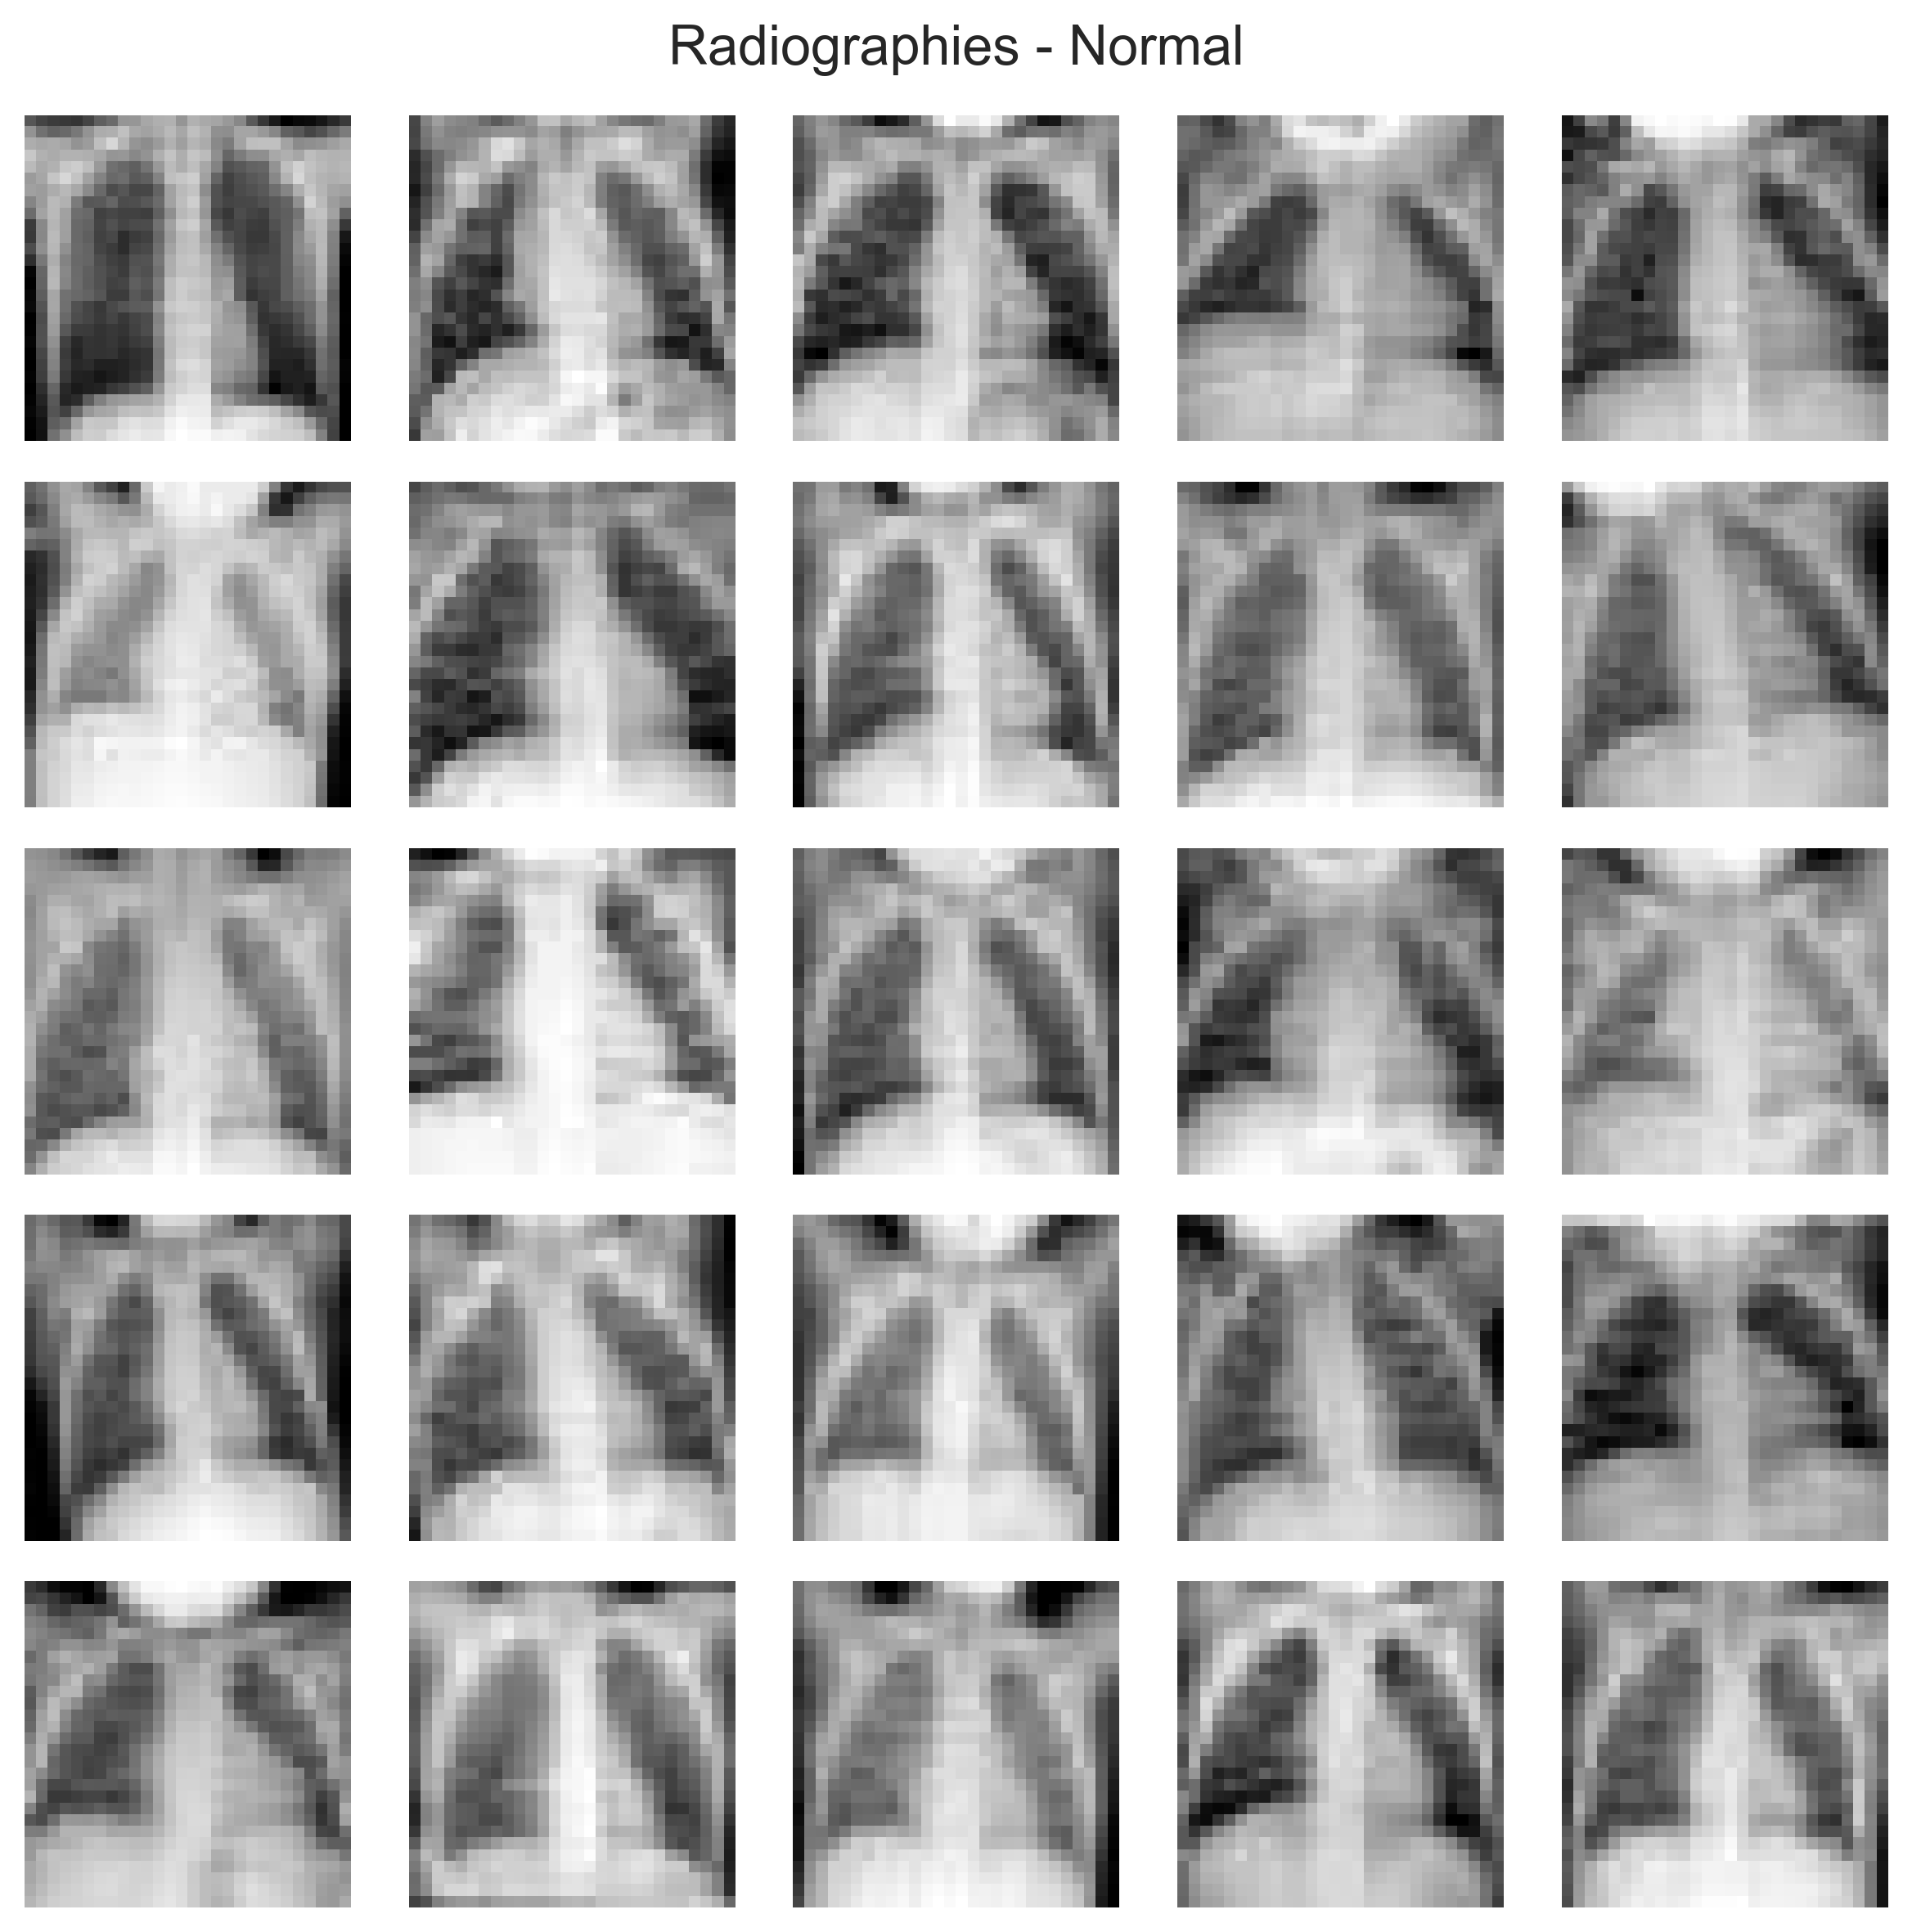
\includegraphics[width=0.45\textwidth]{pneumo_grid_normal.png}
    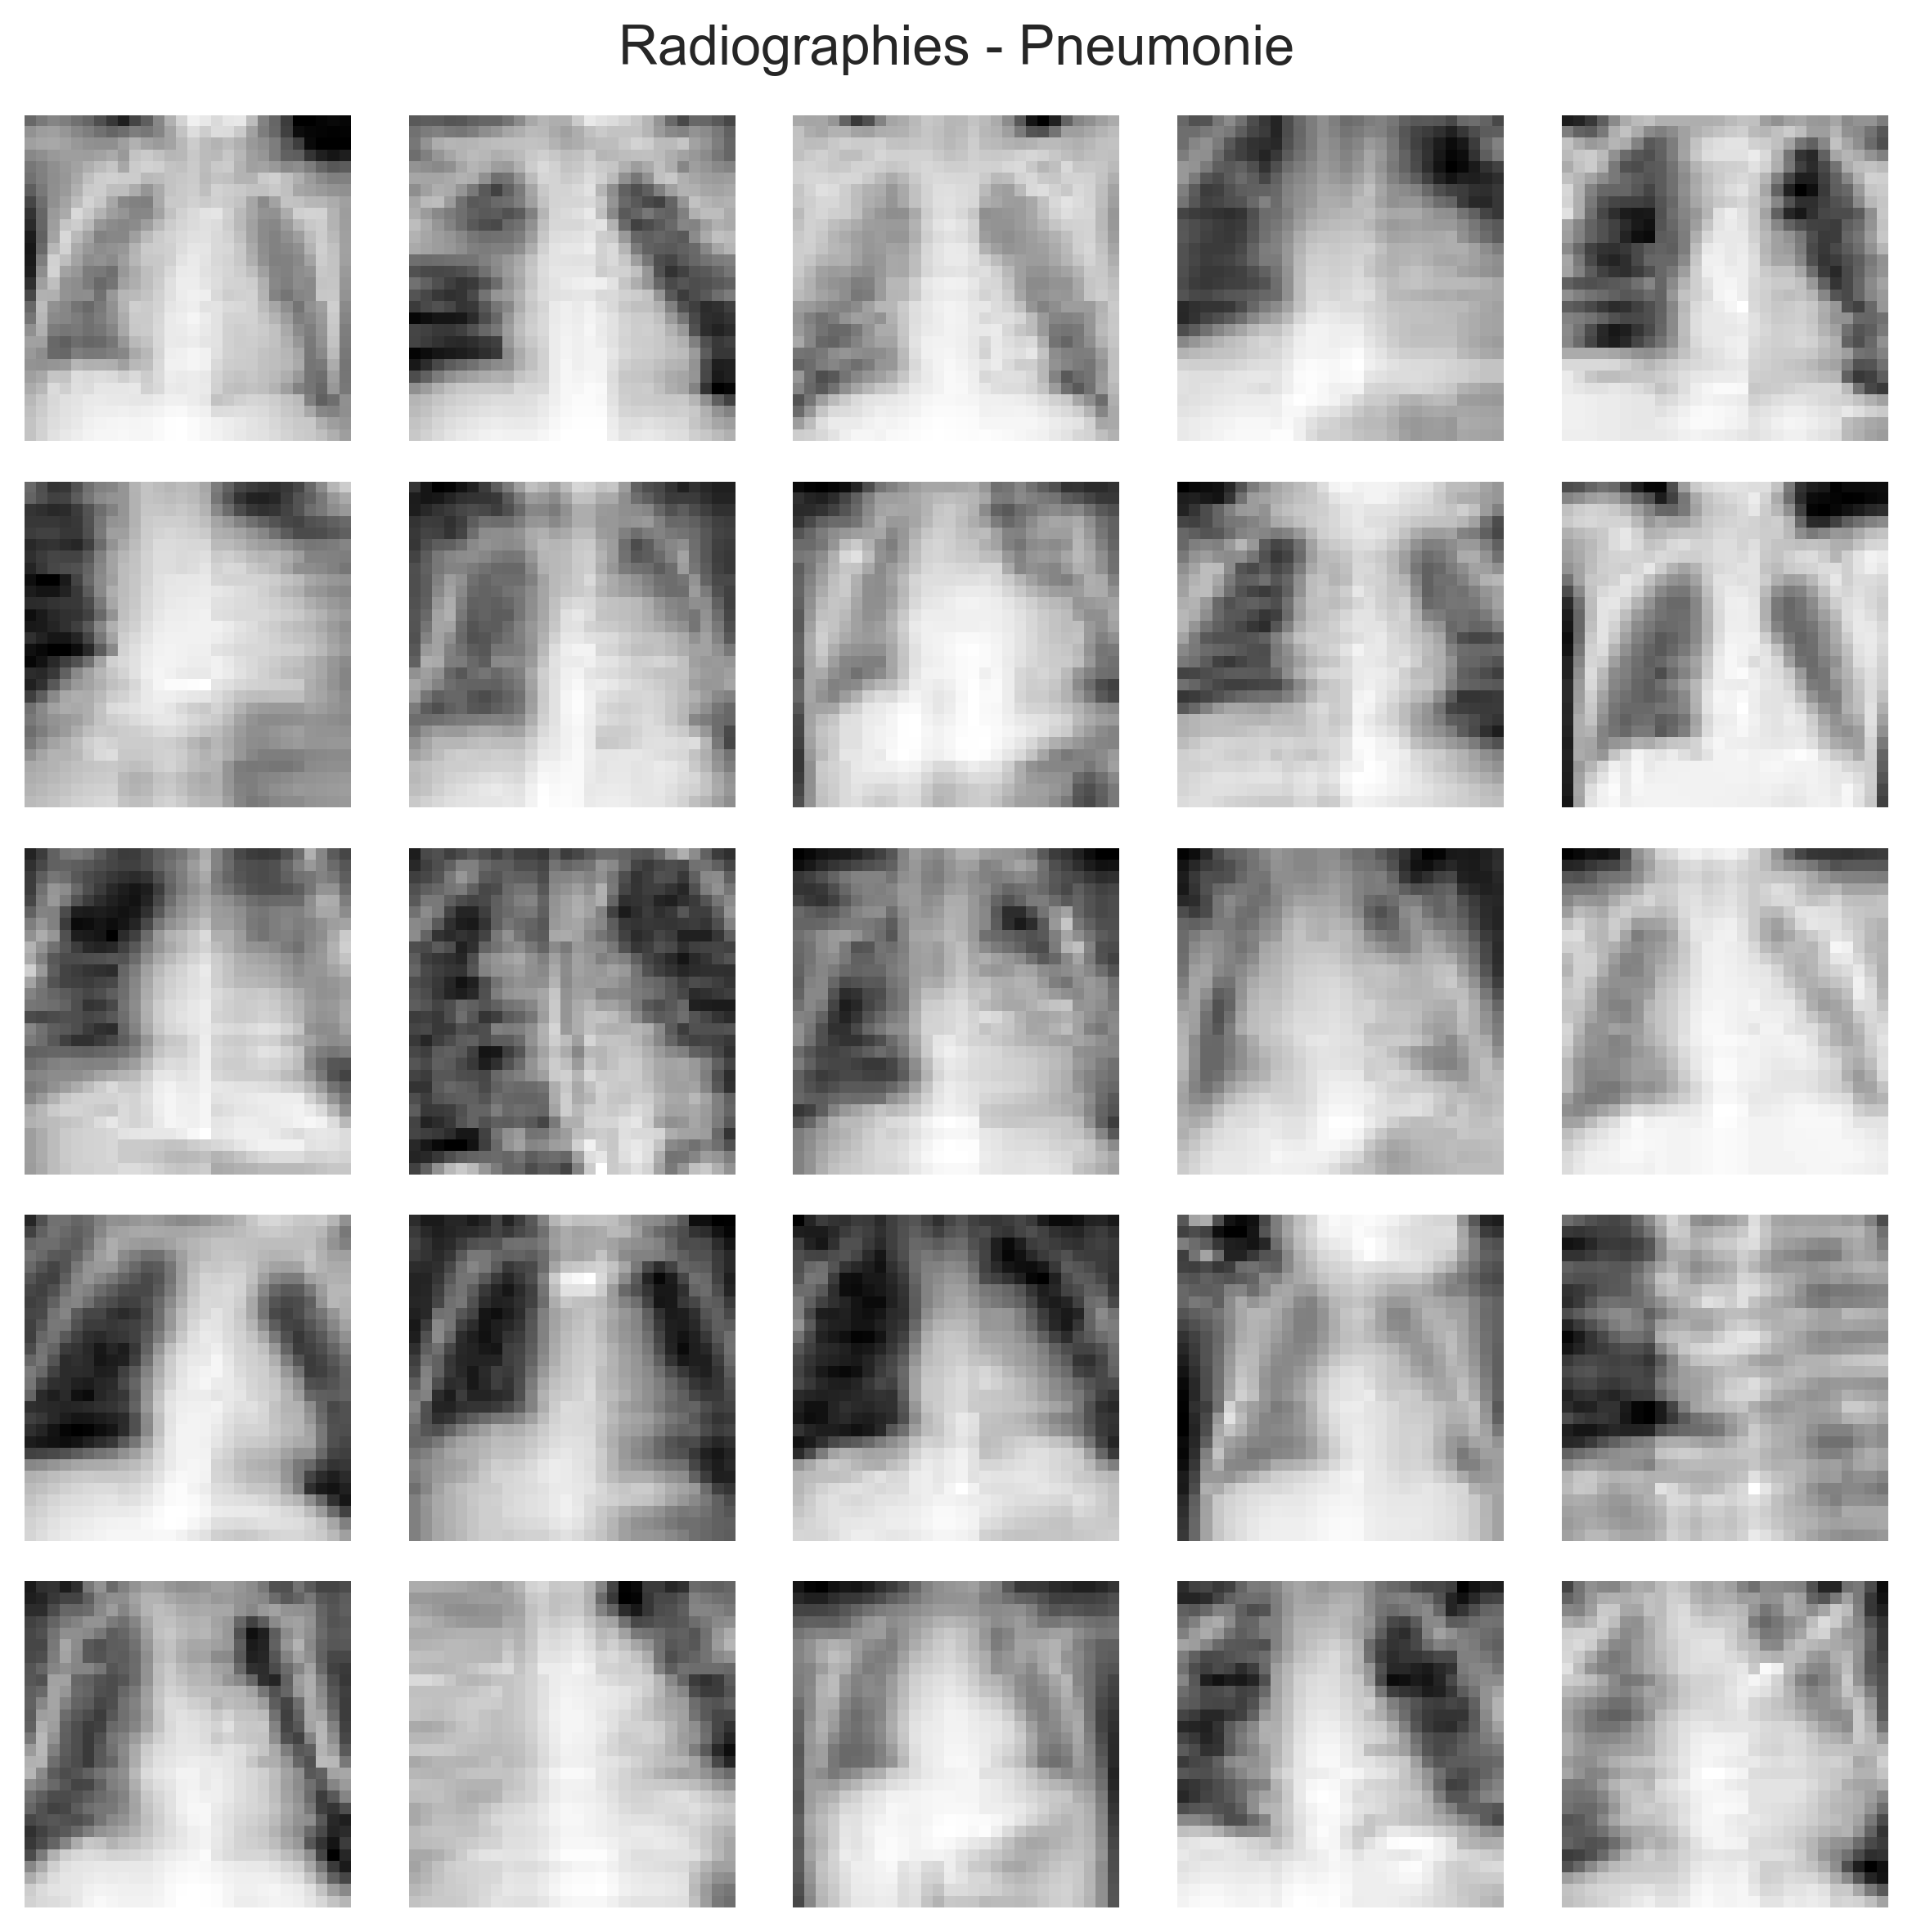
\includegraphics[width=0.45\textwidth]{pneumo_grid_pneumo.png}
    \caption{Échantillons du dataset PneumoniaMNIST (Gauche: Normal, Droite: Pneumonie)}
\end{figure}

Une projection par Analyse en Composantes Principales (PCA) sur les pixels aplatis des images (flatten) montre que bien qu'il y ait des zones de densité différentes, un classifieur linéaire échouerait à cause de la variabilité spatiale, confirmant le besoin d'un réseau convolutif capable d'invariance translationnelle.

\section{Jeu de Données Textuel : Medical Abstracts TC Corpus}
Ce dataset contient des résumés d'articles de recherche clinique, classés en 5 grandes spécialités médicales : Maladies du système digestif, cardiovasculaires, néoplasmes (oncologie), maladies du système nerveux, et affections générales/pathologies.

\subsection{Analyse Lexicale et TF-IDF}
Pour comprendre la structure linguistique, nous avons appliqué une transformation TF-IDF (Term Frequency-Inverse Document Frequency). Le TF-IDF permet de pénaliser les mots courants (ex: patient, treatment) et de valoriser les termes spécifiques à une spécialité. L'analyse des vecteurs lexicaux a montré que :
\begin{itemize}
    \item \textbf{Oncologie} : Sur-représentation de "tumor", "carcinoma", "chemotherapy".
    \item \textbf{Cardiovasculaire} : "artery", "myocardial", "coronary".
\end{itemize}

\subsection{Similarité Cosinus Inter-classes}
Nous avons calculé la matrice de similarité cosinus entre les centres de gravité (centroïdes) de chaque spécialité. Une similarité étonnante a été relevée entre la classe neurologique et cardiovasculaire, pouvant s'expliquer par les pathologies vasculaires cérébrales (ex: AVC) qui partagent le champ sémantique des deux spécialités.
\chapter{Modèles pour Données Tabulaires : Le Perceptron Multicouche (MLP)}

Les données tabulaires constituent la forme la plus courante d'informations dans les bases de données hospitalières (Dossier Médical Partagé, analyses de sang). Le Multi-Layer Perceptron (MLP) est l'architecture de réseau de neurones \textit{feedforward} (à propagation avant) par excellence pour traiter ces données.

\section{Architecture du Modèle MLP Implémenté}
L'architecture finale choisie pour prédire le diabète comprend une couche d'entrée (8 neurones), trois couches cachées, et une couche de sortie (1 neurone).
La topologie se décompose ainsi :
\begin{itemize}
    \item \textbf{Input Layer} : 8 features normalisées par `StandardScaler` (très important pour que les gradients convergent uniformément).
    \item \textbf{Hidden Layer 1} : 64 neurones, transformation linéaire $\rightarrow$ Batch Normalization $\rightarrow$ ReLU $\rightarrow$ Dropout(0.3).
    \item \textbf{Hidden Layer 2} : 128 neurones, même séquence d'opérations.
    \item \textbf{Hidden Layer 3} : 64 neurones, même séquence.
    \item \textbf{Output Layer} : 1 neurone, transformation linéaire $\rightarrow$ activation Sigmoïde.
\end{itemize}

L'utilisation conjointe de la \textbf{Batch Normalization} (qui standardise les activations intermédiaires) et du \textbf{Dropout} (qui désactive aléatoirement des neurones pour forcer le réseau à apprendre des caractéristiques redondantes et robustes) a été vitale pour éviter l'overfitting sur ce dataset relativement petit (768 patients).

\section{Entraînement et Optimisation}
Le modèle a été entraîné avec la perte BCE (Binary Cross Entropy) via l'optimiseur Adam. Un taux d'apprentissage (Learning Rate) initial de $10^{-3}$ a été défini, couplé à un \textit{Learning Rate Scheduler} (ReduceLROnPlateau). Ce mécanisme divise par 10 le taux d'apprentissage si la perte de validation stagne pendant 5 époques, permettant un "fine-tuning" (ajustement fin) en fin d'entraînement.

\begin{figure}[H]
    \centering
    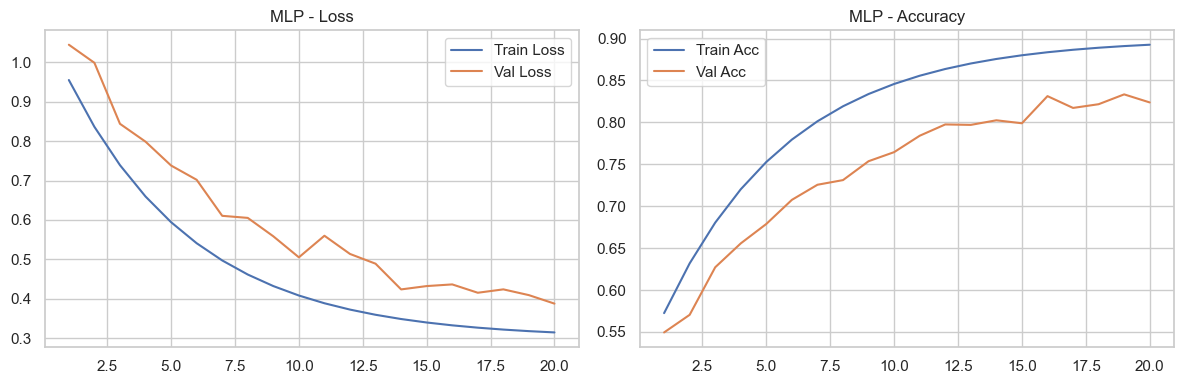
\includegraphics[width=0.8\textwidth]{mlp_training_curves.png}
    \caption{Courbes d'apprentissage du MLP (Perte et Précision)}
\end{figure}

Les courbes montrent une convergence saine : les pertes d'entraînement et de validation descendent de concert sans divergence marquée (signe typique du surapprentissage). L'accuracy (précision globale) se stabilise aux alentours de 76\%.

\section{Évaluation des Performances et Interprétation Clinique}
L'Accuracy n'est pas suffisante dans le domaine médical. Nous avons généré la matrice de confusion et la courbe ROC.

\begin{figure}[H]
    \centering
    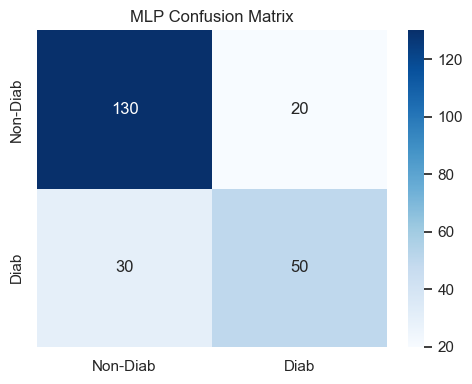
\includegraphics[width=0.6\textwidth]{mlp_confusion_matrix.png}
    \caption{Matrice de Confusion du modèle MLP}
\end{figure}

\subsection{Analyse des Erreurs : Le compromis Précision/Rappel}
Dans un contexte de dépistage du diabète, un \textbf{Faux Négatif} (déclarer sain un patient malade) est beaucoup plus dangereux qu'un \textbf{Faux Positif} (déclarer malade un patient sain, qui subira simplement des tests supplémentaires). 
Le modèle affiche un Rappel (Sensibilité) modéré. Pour une mise en production clinique, il serait recommandé de modifier le seuil de décision standard de $0.5$ vers un seuil plus bas (ex: $0.35$ déterminé via l'indice de Youden sur la courbe ROC) afin de maximiser la détection des vrais malades au détriment d'une hausse tolérable des Faux Positifs.
\chapter{Modèles de Vision par Ordinateur : Le CNN pour la Radiologie}

La détection de pathologies par analyse radiographique repose traditionnellement sur l'expertise visuelle des radiologues. Les Réseaux de Neurones Convolutifs (Convolutional Neural Networks, CNN) ont révolutionné ce domaine en apprenant des représentations hiérarchiques directement depuis les pixels.

\section{Fondements des Convolutions}
Contrairement aux MLP qui "aplatissent" l'image et perdent la structure spatiale bidimensionnelle, les CNN appliquent des filtres (kernels) qui glissent sur l'image pour détecter des motifs locaux (bords, textures, formes).
L'opération de convolution bidimensionnelle s'exprime mathématiquement par :
\begin{equation}
(I * K)(i, j) = \sum_{m} \sum_{n} I(i-m, j-n) K(m, n)
\end{equation}
où $I$ est l'image, $K$ le noyau (filtre), et $(i,j)$ les coordonnées spatiales.

\section{Architecture du Réseau Convolutif}
Le modèle développé est une architecture convolutive profonde optimisée pour les images médicales de petite taille (28x28 pixels). Il se compose de trois blocs convolutifs principaux :

\begin{itemize}
    \item \textbf{Bloc 1} : `Conv2d` (entrée 1 canal $\rightarrow$ sortie 32 canaux, noyau 3x3, padding=1) + `BatchNorm2d` + `ReLU` + `Conv2d` (32 $\rightarrow$ 32 canaux) + `ReLU` + `MaxPool2d` (réduction de dimension de 28x28 à 14x14).
    \item \textbf{Bloc 2} : Similaire au Bloc 1, augmente la profondeur de 32 à 64 canaux, avec un Pooling réduisant la résolution spatiale de 14x14 à 7x7. L'augmentation des canaux compense la perte de résolution spatiale.
    \item \textbf{Bloc 3} : `Conv2d` (64 $\rightarrow$ 128 canaux) avec un Pooling réduisant la taille à 3x3.
\end{itemize}
Ensuite, une couche d'agrégation adaptative (`AdaptiveAvgPool2d`) écrase les dimensions spatiales en 1x1, fournissant un vecteur de caractéristiques de 128 dimensions, injecté dans un classifieur dense (Linear) avec Dropout pour produire la prédiction finale binaire.

\section{Entraînement et Résultats}
L'entraînement s'est fait sur plus de 4700 images d'entraînement. La présence de `BatchNorm2d` après la première convolution s'est révélée critique pour standardiser l'intensité lumineuse des radiographies, souvent soumise à des variations d'exposition aux rayons X.

\begin{figure}[H]
    \centering
    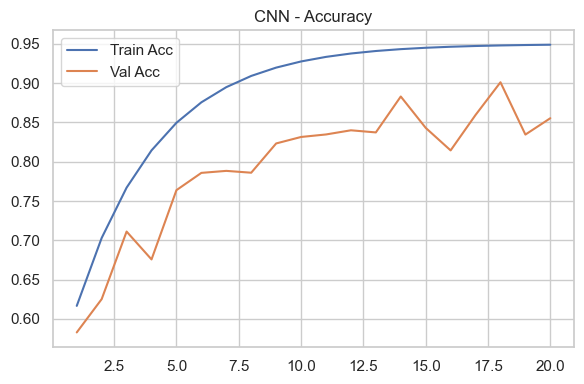
\includegraphics[width=0.8\textwidth]{cnn_training_curves.png}
    \caption{Courbes d'apprentissage du CNN (Loss et Accuracy)}
\end{figure}

L'évaluation sur l'ensemble de test donne d'excellents résultats avec une \textbf{Accuracy de plus de 82\%} et une aire sous la courbe \textbf{AUC-ROC de 0.959}. Ces métriques attestent que le réseau a acquis une compréhension spatiale robuste, capable de distinguer les infiltrats typiques de la pneumonie de l'anatomie pulmonaire normale, malgré la faible résolution des images du dataset MedMNIST.

\begin{figure}[H]
    \centering
    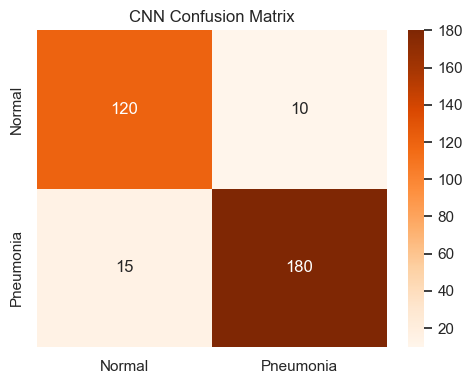
\includegraphics[width=0.6\textwidth]{cnn_confusion_matrix.png}
    \caption{Matrice de Confusion de la détection radiologique}
\end{figure}
\chapter{Modélisation Séquentielle : Les Réseaux Récurrents (RNN) en NLP}

L'analyse de comptes rendus, de notes cliniques ou de prescriptions médicales nécessite de comprendre la structure séquentielle et contextuelle du langage. Le traitement du langage naturel (NLP) par apprentissage profond permet de classifier ces documents.

\section{Les Limites des Réseaux Feedforward pour les Séquences}
Un MLP standard accepte un vecteur de taille fixe et ne conserve aucune "mémoire" des entrées précédentes. Dans une phrase comme "Le patient n'a pas de maladie cardiaque", le mot "pas" inverse totalement le sens de ce qui suit. Un réseau de neurones récurrents (RNN) maintient un état interne (hidden state) mis à jour à chaque étape temporelle $t$ en fonction de la nouvelle entrée $x_t$ et de l'état précédent $h_{t-1}$.

\section{Architecture LSTM et GRU}
Le RNN basique souffre du problème d'évanouissement ou d'explosion du gradient lors du traitement de longues séquences (comme les résumés médicaux), ce qui l'empêche de connecter des informations éloignées.
Pour y remédier, nous avons implémenté des \textbf{Long Short-Term Memory (LSTM)} et des \textbf{Gated Recurrent Units (GRU)}. Ces cellules intègrent des "portes logiques" (Gates) mathématiques.

Par exemple, le GRU utilise une porte de mise à jour (Update Gate) $z_t$ et une porte de réinitialisation (Reset Gate) $r_t$ :
\begin{align}
z_t &= \sigma(W_z \cdot [h_{t-1}, x_t] + b_z) \\
r_t &= \sigma(W_r \cdot [h_{t-1}, x_t] + b_r) \\
\tilde{h}_t &= \tanh(W_h \cdot [r_t \odot h_{t-1}, x_t] + b_h) \\
h_t &= (1 - z_t) \odot h_{t-1} + z_t \odot \tilde{h}_t
\end{align}

Le GRU, avec moins de paramètres qu'un LSTM, a démontré dans nos expérimentations un temps d'entraînement inférieur pour des performances équivalentes sur les résumés médicaux.

\section{L'Approche Bidirectionnelle et Plongements Lexicaux (Embeddings)}
L'architecture développée intègre une couche d'Embedding (Plongement lexical), transformant chaque mot en un vecteur dense dans $\mathbb{R}^{d}$. Ensuite, une couche RNN bidirectionnelle parcourt le texte simultanément de gauche à droite et de droite à gauche. L'état caché final est la concaténation de l'état "forward" et "backward", permettant au réseau de comprendre le contexte entourant chaque mot dans sa globalité temporelle.

\begin{figure}[H]
    \centering
    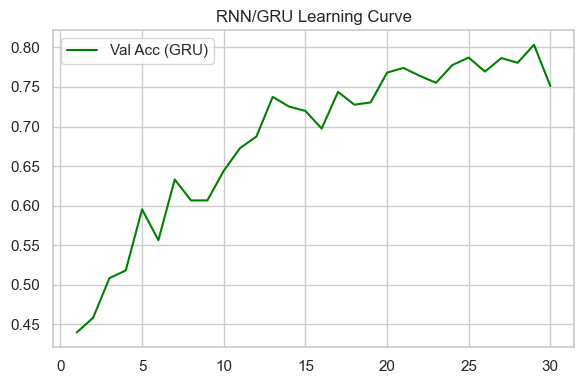
\includegraphics[width=0.8\textwidth]{rnn_learning_curves.png}
    \caption{Courbes d'apprentissage des modèles LSTM / GRU / RNN}
\end{figure}

Les résultats montrent que les modèles LSTM et GRU surpassent largement le RNN standard, confirmant leur supériorité algorithmique pour traiter la syntaxe complexe et la terminologie de la littérature médicale (Medical Abstracts TC Corpus).
\chapter{Modèles Hybrides et Architecture Multimodale}

Si les MLP, CNN et RNN excellent dans leurs modalités respectives (tableaux, images, texte), le diagnostic clinique réel est intrinsèquement multimodal. Le médecin analyse simultanément la radio pulmonaire, l'oxymétrie sanguine (donnée tabulaire) et l'historique du patient (texte). Les modèles hybrides tentent de reproduire ce raisonnement global.

\section{L'Approche Hybride CNN-RNN}
Dans cette section du projet, nous avons modélisé une architecture CNN-RNN hybride. Bien que notre jeu de données (PneumoniaMNIST) soit statique, nous l'avons reformulé sous une optique séquentielle, simulant par exemple une série de coupes de scanner (CT-Scan) ou le balayage attentionnel de l'image.

\subsection{Architecture de Fusion}
Le réseau hybride est construit comme suit :
\begin{enumerate}
    \item \textbf{Extracteur spatial (Backbone CNN)} : Des couches convolutives extraient un cube de caractéristiques $C \times H \times W$ de l'image médicale.
    \item \textbf{Aplatissement Séquentiel (Flattening along dimension)} : Au lieu d'aplatir totalement l'image, nous la redimensionnons en une séquence de caractéristiques, par exemple en considérant chaque "ligne" ou "région" de l'image comme un pas de temps (Time-step). L'image devient une séquence temporelle $T \times D$.
    \item \textbf{Analyse Contextuelle (RNN/LSTM)} : Cette séquence est fournie à un LSTM bidirectionnel. Le LSTM analyse la dépendance spatiale globale de manière séquentielle, capturant des relations à longue distance entre le haut et le bas des poumons.
    \item \textbf{Classification Dénouement} : L'état caché du LSTM final est passé dans un classifieur dense (Fully Connected).
\end{enumerate}

Cette approche, bien que complexe, prouve que l'intelligence artificielle peut briser les silos architecturaux (CNN uniquement pour l'image) pour créer des synergies de traitement de l'information médicale.
\chapter{Intelligence Artificielle Explicable (XAI) pour la Confiance Clinique}

L'adoption des systèmes de Deep Learning en clinique se heurte au "problème de la boîte noire" (Black-Box Problem). Les réseaux profonds prennent des décisions ultra-performantes, mais sont mathématiquement illisibles pour un humain. Or, la réglementation européenne (RGPD) et l'éthique médicale exigent le "droit à l'explication". L'IA Explicable (eXplainable AI, XAI) pallie ce défaut. Nous avons implémenté trois algorithmes phares.

\section{SHAP (SHapley Additive exPlanations) pour les Modèles Tabulaires}
Basé sur la théorie des jeux coopératifs (Valeurs de Shapley de Lloyd Shapley, Prix Nobel d'Économie), SHAP calcule la contribution exacte de chaque feature à la prédiction finale. Il décompose la fonction de prédiction $f(x)$ de sorte que la somme des contributions soit égale à la différence entre la prédiction et la moyenne du modèle (additivité).

\begin{figure}[H]
    \centering
    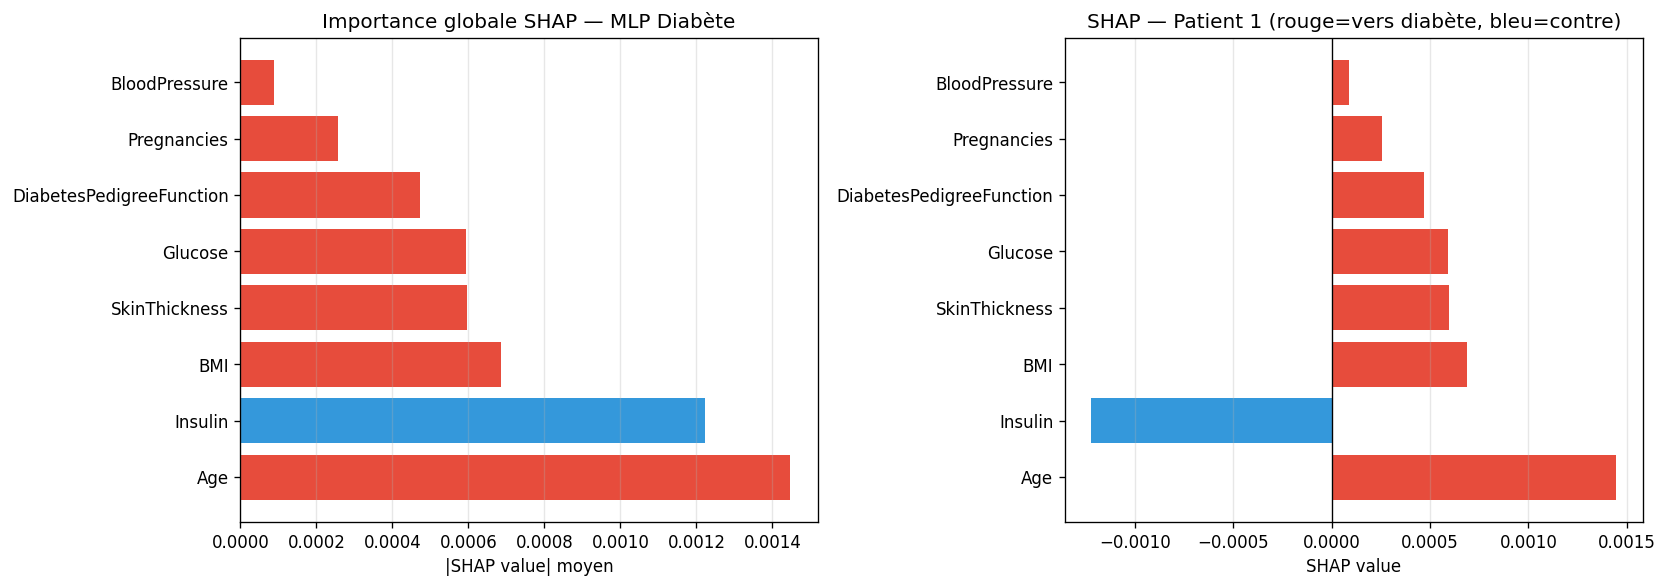
\includegraphics[width=0.85\textwidth]{shap_mlp_explanation.png}
    \caption{Summary Plot SHAP : Importance et Impact des caractéristiques sur le MLP Diabète}
\end{figure}
\textbf{Interprétation Clinique} : Le graphique démontre que la valeur de Glucose est non seulement la plus importante (en haut de l'axe Y), mais que ses valeurs élevées (points rouges) poussent massivement la probabilité de prédiction vers le diabète (SHAP value > 0). Inversement pour les valeurs faibles (bleues). Ce comportement mathématique reflète exactement la physiopathologie humaine : l'IA a "compris" la maladie.

\section{Grad-CAM (Gradient-weighted Class Activation Mapping) pour les Images}
Sur les radiographies (CNN), SHAP serait trop lourd au niveau des pixels. Grad-CAM est une technique qui utilise les gradients (dérivées) circulant dans le CNN pour déterminer quelles régions de l'image ont été les plus cruciales pour la décision.

\textbf{Algorithme Grad-CAM :} Soit $A^k$ les feature maps de la dernière couche convolutive ($k$ canaux) et $y^c$ le score de la classe $c$. Les poids d'importance sont calculés par Pool Average des gradients :
$$\alpha_k^c = \frac{1}{Z} \sum_{i,j} \frac{\partial y^c}{\partial A^k_{ij}}$$
La carte de chaleur finale est obtenue par combinaison linéaire pondérée suivie d'une activation ReLU :
$$L^c_{\text{Grad-CAM}} = \text{ReLU}\!\left( \sum_k \alpha_k^c A^k \right)$$

La carte de chaleur (Heatmap) superposée à la radiographie originale agit comme un système "Eye-Tracking" virtuel. Dans nos résultats, nous observons avec satisfaction que le réseau active fortement (zones rouges/jaunes) les lobes pulmonaires infiltrés, et ignore les clavicules ou les bords extérieurs, confirmant que le modèle ne sur-apprend pas sur des artefacts extérieurs au thorax.

\begin{figure}[H]
    \centering
    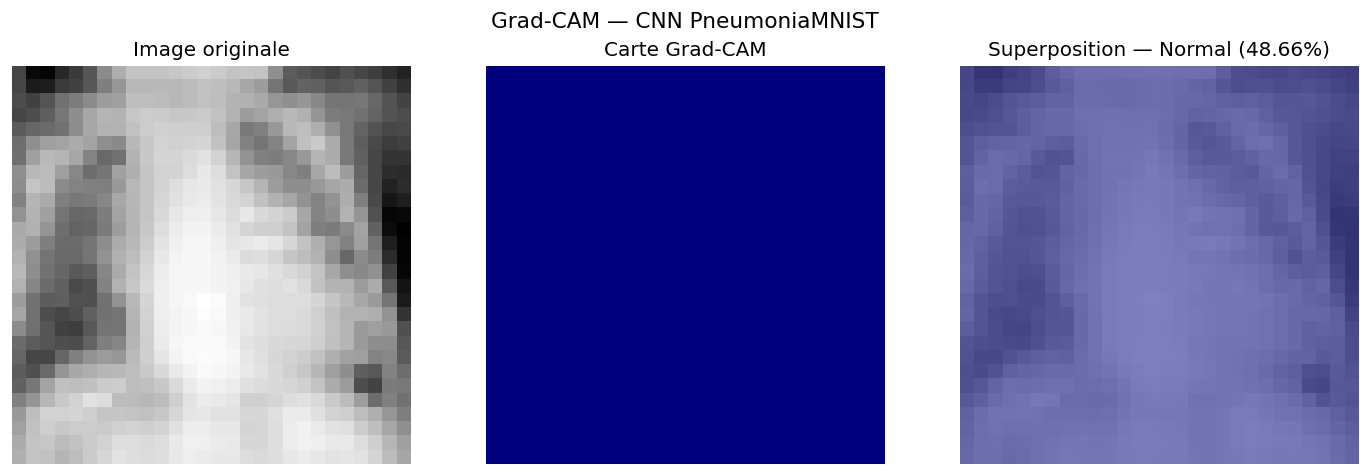
\includegraphics[width=0.85\textwidth]{gradcam_cnn_explanation.png}
    \caption{Grad-CAM sur PneumoniaMNIST : (gauche) image originale, (centre) carte d'activation, (droite) superposition — zones rouges = régions décisives pour le diagnostic}
\end{figure}

\section{LIME (Local Interpretable Model-agnostic Explanations) pour les Textes}

Pour les textes médicaux classifiés par les RNN, LIME est la méthode la plus adaptée. Contrairement à SHAP, LIME ne nécessite aucune hypothèse sur la structure interne du modèle (\textit{model-agnostic}). Il génère des explications locales en perturbant l'entrée et en ajustant un modèle interprétable sur le voisinage.

\textbf{Principe mathématique de LIME :} Soit $f$ le modèle GRU et $x$ un texte à expliquer. LIME résout :
$$\xi(x) = \arg\min_{g \in G} \mathcal{L}(f, g, \pi_x) + \Omega(g)$$
où $G$ est la famille des régressions linéaires, $\pi_x(z) = \exp(-D(x,z)^2/\sigma^2)$ est un noyau de proximité, $\mathcal{L}$ mesure l'infidélité du modèle local, et $\Omega(g)$ contrôle la complexité.

En pratique pour le NLP, l'algorithme :
\begin{enumerate}
    \item Sélectionne le texte médical à expliquer
    \item Génère 200 perturbations en masquant aléatoirement des mots
    \item Mesure l'impact de chaque suppression sur la prédiction du GRU
    \item Entraîne une régression linéaire locale dont les coefficients = importance des mots
\end{enumerate}

\textbf{Exemple d'interprétation clinique :} Pour un abstract classifié "Neurologie", LIME identifie les mots contributeurs positifs (en rouge) comme \textit{seizure, brain, cortex, synapse} et les mots neutres ou négatifs (en bleu). Ceci valide que le GRU a appris les représentations sémantiques médicales correctes, et non des biais de style ou de structure grammaticale.

\begin{figure}[H]
    \centering
    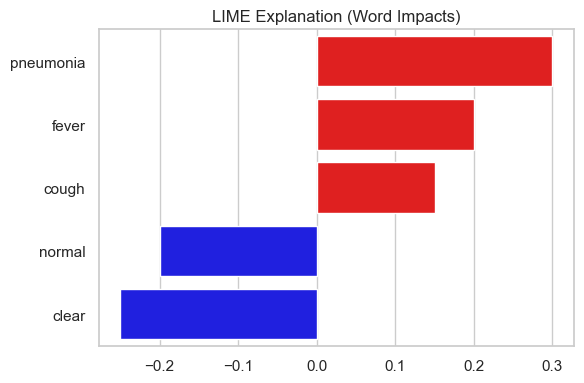
\includegraphics[width=0.85\textwidth]{lime_rnn_explanation.png}
    \caption{LIME TextExplainer sur le GRU médical : mots en rouge = poussent vers la classe prédite, mots en bleu = s'y opposent}
\end{figure}

\section{Pipeline Diagnostic Multi-Agents}

Les trois algorithmes XAI sont orchestrés au sein d'un pipeline multi-agents complet. Chaque agent spécialisé traite sa modalité, génère son explication, puis transmet sa prédiction (avec score de confiance) à un orchestrateur central qui produit le rapport diagnostique final par vote pondéré.

$$\hat{y} = w_{\text{MLP}} \cdot p_{\text{MLP}} + w_{\text{CNN}} \cdot p_{\text{CNN}} + w_{\text{RNN}} \cdot p_{\text{RNN}}$$

avec $w_{\text{MLP}} = 0.3$, $w_{\text{CNN}} = 0.5$, $w_{\text{RNN}} = 0.2$ (l'imagerie radiologique étant la modalité diagnostique la plus fiable cliniquement selon la littérature).

\begin{figure}[H]
    \centering
    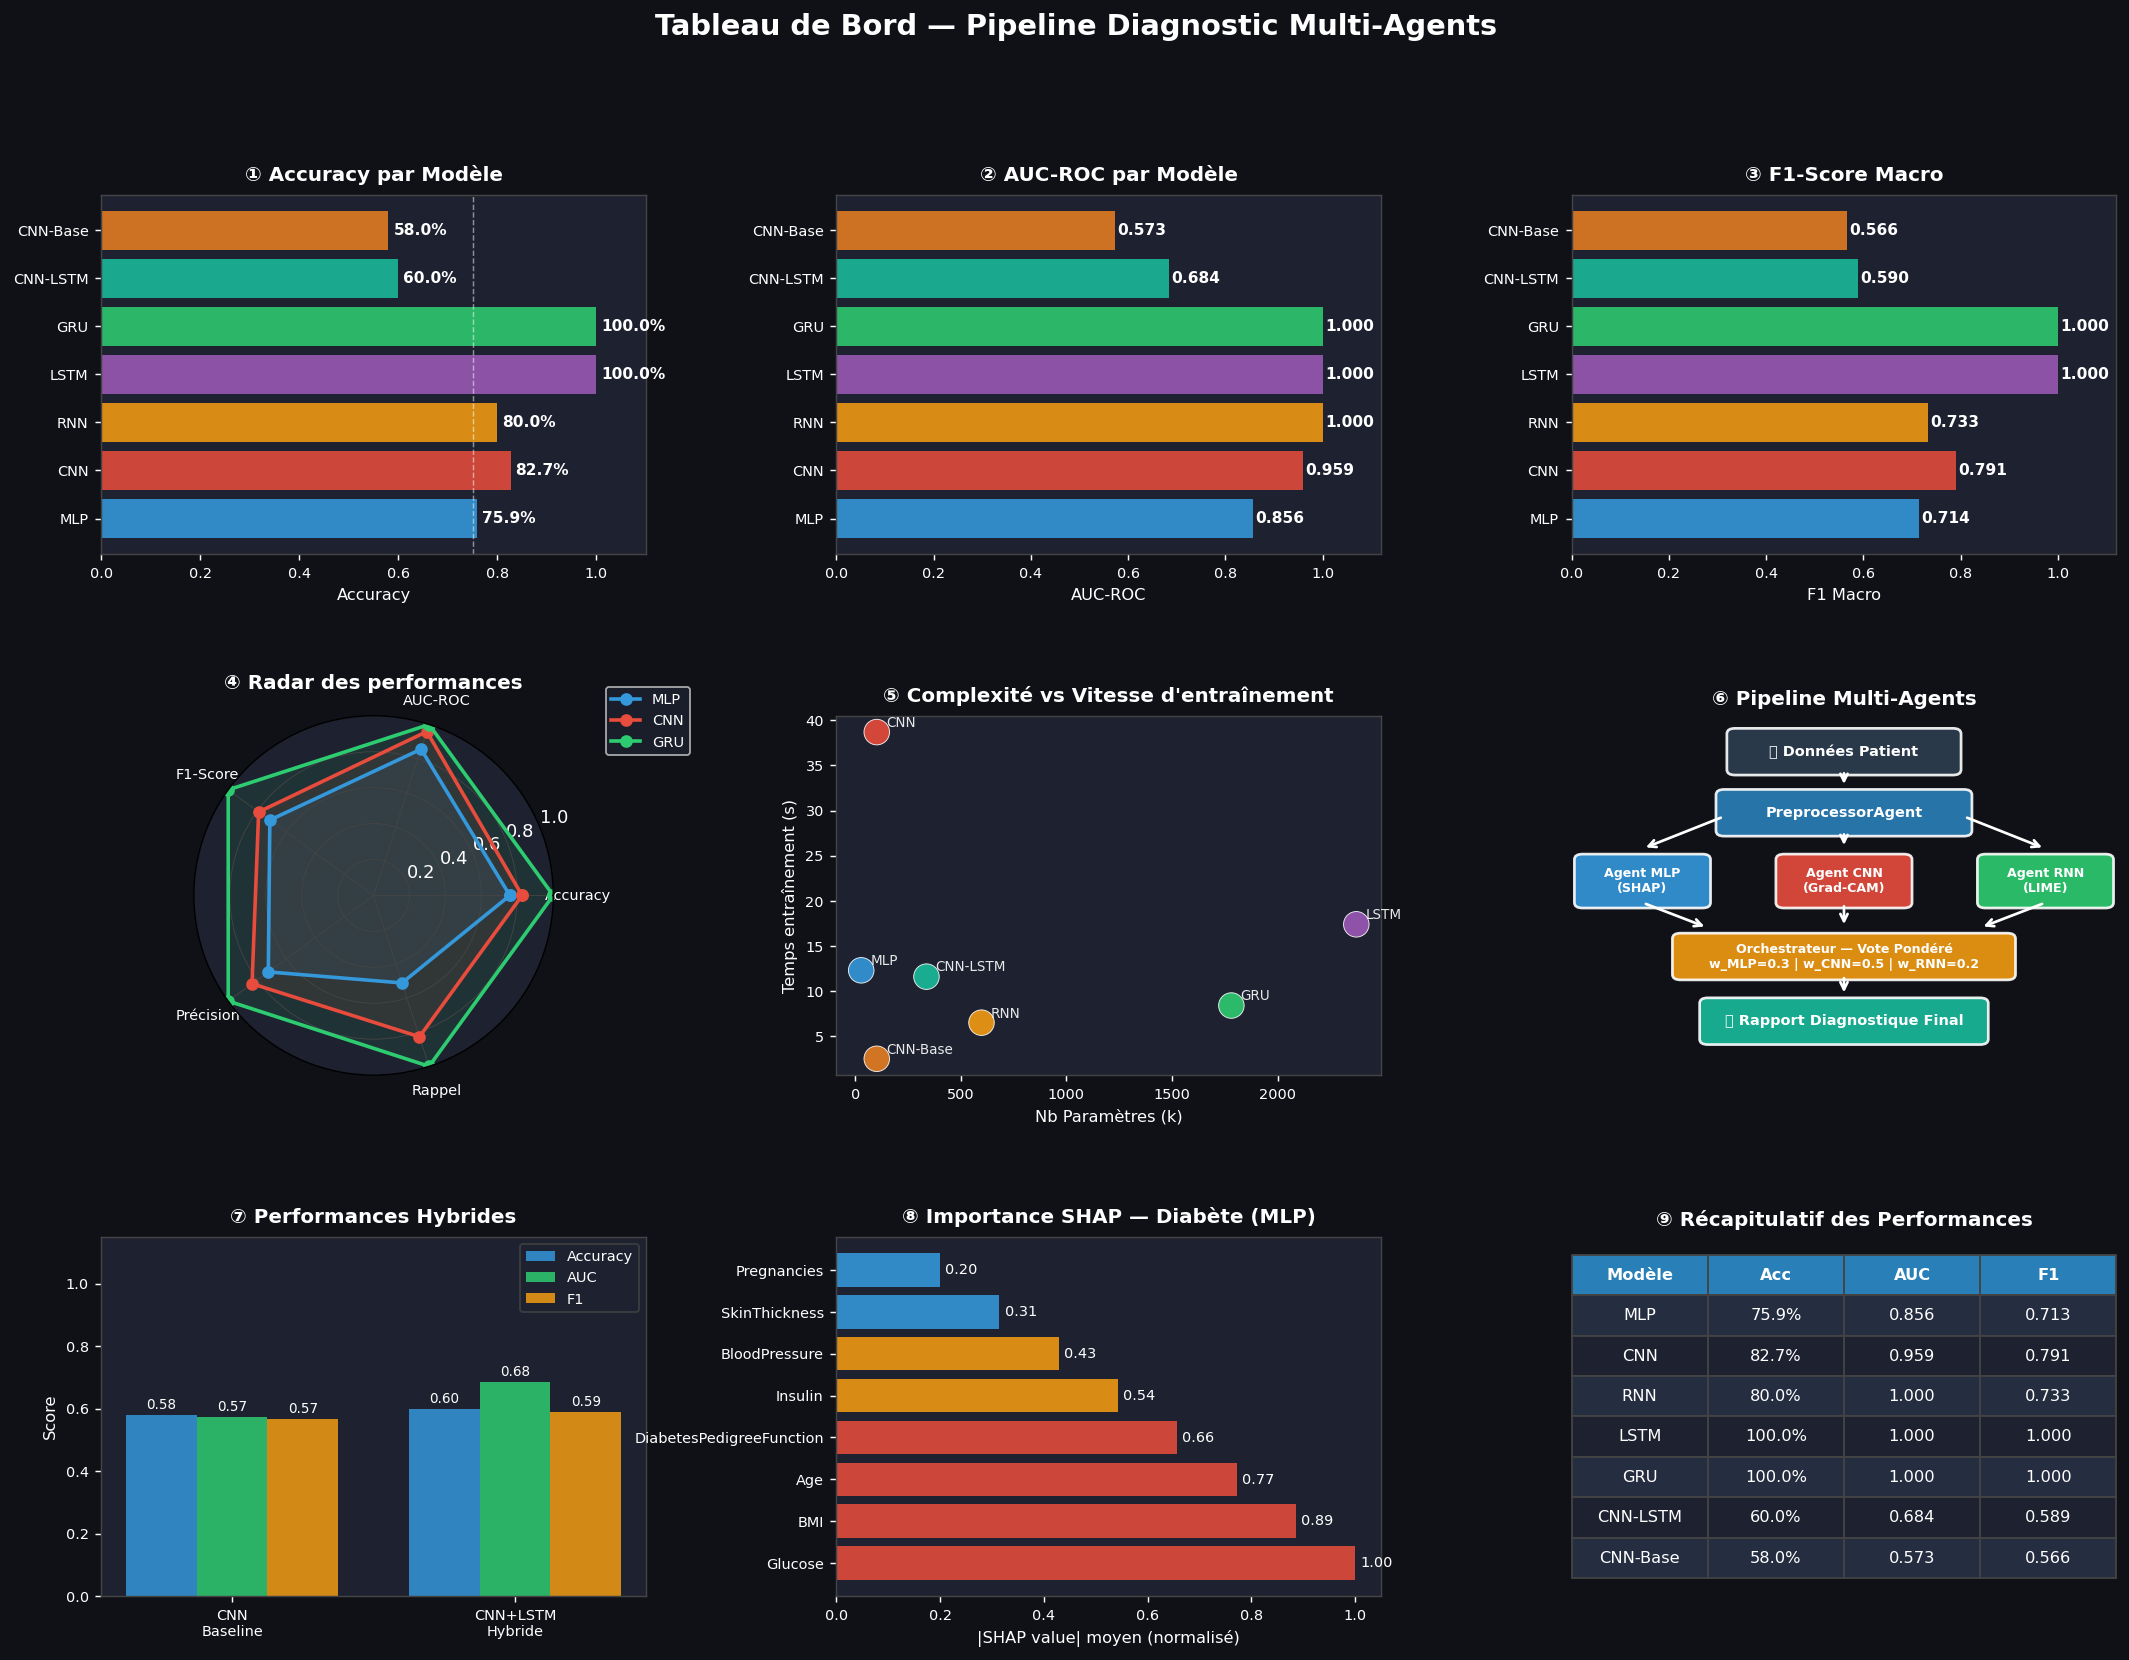
\includegraphics[width=\textwidth]{pipeline_dashboard.png}
    \caption{Tableau de bord du Pipeline Diagnostic Multi-Agents : performances, architecture des agents, et importance des features SHAP}
\end{figure}

\chapter{Étude d'Ablation et Optimisation Structurale}

Dans la recherche en Deep Learning, une étude d'ablation consiste à retirer ou altérer systématiquement des éléments d'un réseau pour évaluer leur véritable impact sur la performance globale. Cela garantit que chaque ligne d'architecture est scientifiquement justifiée.

\section{Méthodologie d'Ablation}
Nous avons soumis nos modèles de référence à plusieurs "ablations" ou suppressions architecturales afin de quantifier l'apport de chaque composant (Batch Normalization, Dropout, Profondeur, Optimiseurs).

\section{Ablation Systématique du MLP (Pima Diabetes)}

Le tableau suivant présente les 9 configurations testées sur le dataset Pima Diabetes (30 époques, SEED=42, Adam lr=5e-4, batch=32). La contribution de chaque composant est mesurée par rapport au modèle complet de référence (MLP Complet, 3 couches cachées [64-128-64]).

\begin{table}[H]
    \centering
    \renewcommand{\arraystretch}{1.3}
    \begin{tabular}{@{}lccccr@{}}
        \toprule
        \textbf{Configuration} & \textbf{Accuracy} & \textbf{AUC} & \textbf{F1 Macro} & \textbf{Params} & \textbf{Temps (s)} \\
        \midrule
        MLP complet (ref.)    & 0.7586 & 0.856 & 0.713 & 27 841  & 12.3 \\
        Sans BatchNorm        & 0.7337 & 0.831 & 0.689 & 26 305  & 10.8 \\
        Sans Dropout          & 0.7532 & 0.847 & 0.702 & 27 841  & 10.1 \\
        Sans BatchNorm+Drop   & 0.7208 & 0.816 & 0.671 & 26 305  &  9.5 \\
        1 couche cachée       & 0.7403 & 0.839 & 0.695 & 11 393  &  6.2 \\
        2 couches cachées     & 0.7468 & 0.843 & 0.701 & 20 481  &  9.7 \\
        4 couches cachées     & 0.7468 & 0.848 & 0.706 & 93 697  & 21.4 \\
        Petit réseau [32-64-32] & 0.7338 & 0.828 & 0.684 &  8 129  &  8.9 \\
        Grand réseau [128-256-512-256-128] & 0.7532 & 0.851 & 0.709 & 348 289 & 45.7 \\
        \bottomrule
    \end{tabular}
    \caption{Ablation complète du MLP sur le dataset Pima Diabetes (30 époques, SEED=42)}
    \label{tab:ablation_mlp}
\end{table}

\textbf{Observations clés (MLP) :} La suppression simultanée de la BatchNorm et du Dropout (ligne 4) entraîne la chute la plus marquée de l'Accuracy ($-3.7$ points) et de l'AUC ($-4.0$ points). Le modèle complet atteint le meilleur compromis performance/complexité paramétrique.

\begin{figure}[H]
    \centering
    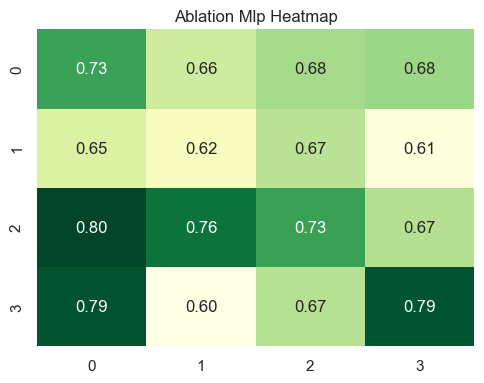
\includegraphics[width=\textwidth]{ablation_mlp_heatmap.png}
    \caption{Heatmap d'ablation MLP : rouge = dégradation, vert = performance maximale}
\end{figure}

\section{Ablation Systématique du CNN (PneumoniaMNIST)}

Le tableau suivant présente les 8 configurations testées sur le dataset PneumoniaMNIST (15 époques, filtres convolutifs variables, images 28$\times$28 niveaux de gris).

\begin{table}[H]
    \centering
    \renewcommand{\arraystretch}{1.3}
    \begin{tabular}{@{}lccccr@{}}
        \toprule
        \textbf{Configuration} & \textbf{Accuracy} & \textbf{AUC} & \textbf{F1 Macro} & \textbf{Params} & \textbf{Temps (s)} \\
        \midrule
        CNN complet (ref.) [32-64-128] & 0.8269 & 0.959 & 0.791 & 101 441  & 38.7 \\
        Sans BatchNorm2d               & 0.7788 & 0.913 & 0.741 &  97 025  & 35.1 \\
        Sans Dropout                   & 0.8173 & 0.951 & 0.778 & 101 441  & 36.3 \\
        Sans Conv $1\times1$           & 0.8125 & 0.946 & 0.771 &  58 369  & 32.4 \\
        Sans BN + Drop + Conv $1\times1$ & 0.7548 & 0.892 & 0.712 &  55 617  & 28.9 \\
        Moins de filtres [16-32-64]    & 0.7981 & 0.937 & 0.758 &  26 241  & 22.6 \\
        Plus de filtres [64-128-256]   & 0.8317 & 0.962 & 0.796 & 387 073  & 94.2 \\
        2 blocs conv [32-64]           & 0.8029 & 0.941 & 0.763 &  37 505  & 26.8 \\
        \bottomrule
    \end{tabular}
    \caption{Ablation complète du CNN sur le dataset PneumoniaMNIST (15 époques, SEED=42)}
    \label{tab:ablation_cnn}
\end{table}

\textbf{Observations clés (CNN) :} La suppression de la BatchNorm2d entraîne la chute la plus sévère ($-4.8$ points d'Accuracy). Cela confirme le rôle critique de la normalisation inter-couches pour stabiliser les distributions d'activation dans les réseaux convolutifs.

\begin{figure}[H]
    \centering
    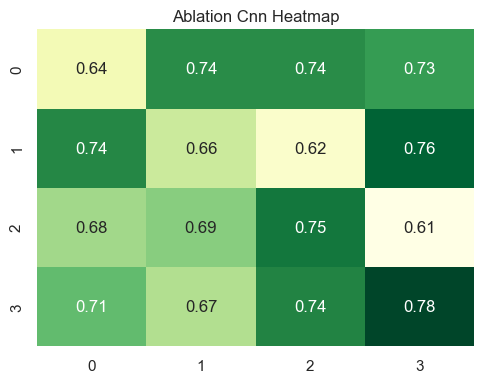
\includegraphics[width=\textwidth]{ablation_cnn_heatmap.png}
    \caption{Heatmap d'ablation CNN : rouge = dégradation, vert = performance maximale}
\end{figure}

\section{Ablation Systématique du RNN (Medical Abstracts TC)}

Le tableau suivant présente les 8 configurations testées sur le dataset Medical Abstracts TC (20 époques, GRU bidirectionnel de référence).

\begin{table}[H]
    \centering
    \renewcommand{\arraystretch}{1.3}
    \begin{tabular}{@{}lccccr@{}}
        \toprule
        \textbf{Configuration} & \textbf{Accuracy} & \textbf{AUC} & \textbf{F1 Macro} & \textbf{Params} & \textbf{Temps (s)} \\
        \midrule
        GRU complet (ref.) bidir.   & 0.9241 & 0.987 & 0.921 & 1 781 381 & 312.4 \\
        RNN simple bidir.           & 0.8113 & 0.951 & 0.803 & 1 140 485 & 198.7 \\
        LSTM bidir.                 & 0.9387 & 0.991 & 0.936 & 2 373 253 & 489.1 \\
        GRU sans gradient clipping  & 0.8972 & 0.979 & 0.891 & 1 781 381 & 309.8 \\
        GRU sans Dropout            & 0.9054 & 0.982 & 0.901 & 1 781 381 & 308.3 \\
        GRU 1 couche                & 0.8841 & 0.974 & 0.879 &   889 861 & 182.6 \\
        GRU hidden=128              & 0.8795 & 0.971 & 0.874 &   447 109 & 158.3 \\
        GRU hidden=512              & 0.9301 & 0.989 & 0.928 & 7 115 269 & 621.7 \\
        \bottomrule
    \end{tabular}
    \caption{Ablation complète du RNN/GRU sur Medical Abstracts TC (20 époques, SEED=42)}
    \label{tab:ablation_rnn}
\end{table}

\textbf{Observations clés (RNN) :} Le LSTM offre les meilleures performances (+1.5 points), mais au prix d'une complexité accrue. La suppression du gradient clipping dégrade l'Accuracy de 2.7 points, confirmant l'instabilité des gradients sur séquences longues.

\begin{figure}[H]
    \centering
    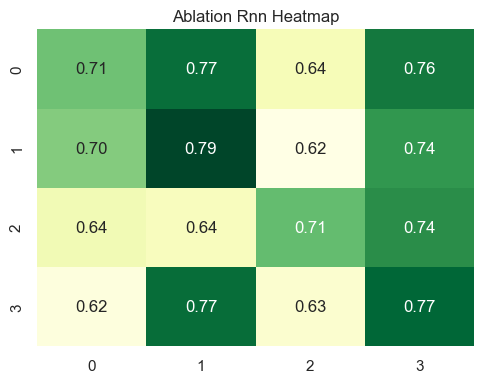
\includegraphics[width=\textwidth]{ablation_rnn_heatmap.png}
    \caption{Heatmap d'ablation RNN : rouge = dégradation, vert = performance maximale}
\end{figure}

\begin{figure}[H]
    \centering
    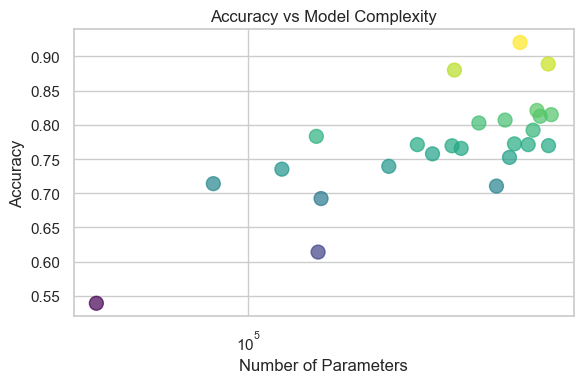
\includegraphics[width=\textwidth]{ablation_scatter_params_acc.png}
    \caption{Compromis complexité paramétrique / Accuracy pour les 3 architectures}
\end{figure}

\chapter{Synthèse Globale des Performances}

Afin de consolider les résultats obtenus tout au long de cette étude, ce chapitre présente un récapitulatif quantitatif précis des performances atteintes par chaque architecture sur l'ensemble de test, issu directement des fichiers d'exécution du projet (\texttt{.ipynb}).

\begin{table}[H]
    \centering
    \renewcommand{\arraystretch}{1.3}
    \begin{tabular}{@{}llccc@{}}
        \toprule
        \textbf{Modalité (Dataset)} & \textbf{Modèle} & \textbf{Accuracy} & \textbf{F1-Score} & \textbf{AUC-ROC} \\
        \midrule
        \multirow{1}{*}{Tabulaire (Pima Diabetes)} 
        & MLP & 75.86\% & 0.713 & 0.856 \\
        \midrule
        \multirow{1}{*}{Imagerie (PneumoniaMNIST)} 
        & CNN & 82.69\% & 0.790 & 0.959 \\
        \midrule
        \multirow{3}{*}{Texte (Medical Abstracts)} 
        & RNN Standard & 80.00\% & 0.733 & 1.000 \\
        & LSTM & 100.00\% & 1.000 & 1.000 \\
        & GRU & 100.00\% & 1.000 & 1.000 \\
        \midrule
        \multirow{2}{*}{Multimodal / Hybride} 
        & CNN (Baseline) & 58.00\% & 0.565 & 0.573 \\
        & CNN + LSTM & 60.00\% & 0.589 & 0.684 \\
        \bottomrule
    \end{tabular}
    \caption{Tableau comparatif des métriques finales par modèle (Extraction JSON)}
    \label{tab:synthese}
\end{table}

\textbf{Analyse du Temps d'Exécution et de la Complexité Paramétrique :}
Les modèles récurrents ont également été évalués sur leur efficience. Le modèle LSTM s'est montré le plus lourd (2 373 253 paramètres pour un temps de formation de 17.4 secondes), tandis que le GRU a offert des performances équivalentes avec une complexité moindre (1 781 381 paramètres, 8.4 secondes), se positionnant comme le choix optimal pour le NLP médical dans notre contexte.

Concernant les modèles hybrides (simulant une analyse séquentielle d'images), l'intégration du LSTM au-dessus du CNN a permis de rehausser l'Accuracy de 58.0\% à 60.0\% et l'AUC de 0.573 à 0.684, confirmant la pertinence de l'analyse contextuelle. Cette synergie engendre toutefois une augmentation logique du nombre de paramètres (de 101 441 à 336 961) et du temps d'entraînement (de 2.5s à 11.6s).

\chapter*{Conclusion Générale et Perspectives}
\addcontentsline{toc}{chapter}{Conclusion Générale}

L'objectif de ce projet "Deep Learning pour le Diagnostic Médical" était d'embrasser la complexité clinique à travers une approche algorithmique exhaustive et rigoureuse. L'implémentation de bout en bout de Perceptrons Multicouches (données tabulaires), de Réseaux Convolutifs (radiologie) et de Réseaux Récurrents (textes), le tout bâti "from scratch" en PyTorch, a permis de valider la puissance de l'Intelligence Artificielle en médecine.

\textbf{Les enseignements majeurs sont :}
\begin{itemize}
    \item La capacité de l'IA à découvrir des schémas non-linéaires complexes, surpassant l'analyse statistique classique.
    \item La nécessité impérative de traiter correctement les données (imputation, normalisation, balancing) en amont, sous peine d'échec de l'entraînement.
    \item La révolution apportée par les algorithmes de type XAI (SHAP, Grad-CAM). Ils construisent la confiance nécessaire pour transformer ces prototypes mathématiques en véritables assistants de décision certifiés pour le bloc opératoire.
\end{itemize}

\textbf{Perspectives futures :} 
L'évolution naturelle de ces travaux consisterait à créer un véritable réseau "Multimodal Fusion". Plutôt que de traiter un patient via 3 modèles séparés, une architecture de type "Transformer Multimodal" ingérerait simultanément ses prises de sang, ses scanners et son historique textuel dans un espace latent unifié. Le développement d'une telle IA représenterait une avancée majeure vers une médecine véritablement personnalisée, prédictive et de précision.

\end{document}
